% Options for packages loaded elsewhere
\PassOptionsToPackage{unicode}{hyperref}
\PassOptionsToPackage{hyphens}{url}
\documentclass[
]{article}
\usepackage{xcolor}
\usepackage[a4paper,margin=0.25in]{geometry}
\usepackage{amsmath,amssymb}
\setcounter{secnumdepth}{5}
\usepackage{iftex}
\ifPDFTeX
  \usepackage[T1]{fontenc}
  \usepackage[utf8]{inputenc}
  \usepackage{textcomp} % provide euro and other symbols
\else % if luatex or xetex
  \usepackage{unicode-math} % this also loads fontspec
  \defaultfontfeatures{Scale=MatchLowercase}
  \defaultfontfeatures[\rmfamily]{Ligatures=TeX,Scale=1}
\fi
% \usepackage{lmodern}
\ifPDFTeX\else
  % xetex/luatex font selection
\fi
% Use upquote if available, for straight quotes in verbatim environments
\IfFileExists{upquote.sty}{\usepackage{upquote}}{}
\IfFileExists{microtype.sty}{% use microtype if available
  \usepackage[]{microtype}
  \UseMicrotypeSet[protrusion]{basicmath} % disable protrusion for tt fonts
}{}
\makeatletter
\@ifundefined{KOMAClassName}{% if non-KOMA class
  \IfFileExists{parskip.sty}{%
    \usepackage{parskip}
  }{% else
    \setlength{\parindent}{0pt}
    \setlength{\parskip}{6pt plus 2pt minus 1pt}}
}{% if KOMA class
  \KOMAoptions{parskip=half}}
\makeatother
\usepackage{color}
\usepackage{fancyvrb}
\newcommand{\VerbBar}{|}
\newcommand{\VERB}{\Verb[commandchars=\\\{\}]}
\DefineVerbatimEnvironment{Highlighting}{Verbatim}{commandchars=\\\{\}}
% Add ',fontsize=\small' for more characters per line
\newenvironment{Shaded}{}{}
\newcommand{\AlertTok}[1]{\textcolor[rgb]{1.00,0.00,0.00}{\textbf{#1}}}
\newcommand{\AnnotationTok}[1]{\textcolor[rgb]{0.38,0.63,0.69}{\textbf{\textit{#1}}}}
\newcommand{\AttributeTok}[1]{\textcolor[rgb]{0.49,0.56,0.16}{#1}}
\newcommand{\BaseNTok}[1]{\textcolor[rgb]{0.25,0.63,0.44}{#1}}
\newcommand{\BuiltInTok}[1]{\textcolor[rgb]{0.00,0.50,0.00}{#1}}
\newcommand{\CharTok}[1]{\textcolor[rgb]{0.25,0.44,0.63}{#1}}
\newcommand{\CommentTok}[1]{\textcolor[rgb]{0.38,0.63,0.69}{\textit{#1}}}
\newcommand{\CommentVarTok}[1]{\textcolor[rgb]{0.38,0.63,0.69}{\textbf{\textit{#1}}}}
\newcommand{\ConstantTok}[1]{\textcolor[rgb]{0.53,0.00,0.00}{#1}}
\newcommand{\ControlFlowTok}[1]{\textcolor[rgb]{0.00,0.44,0.13}{\textbf{#1}}}
\newcommand{\DataTypeTok}[1]{\textcolor[rgb]{0.56,0.13,0.00}{#1}}
\newcommand{\DecValTok}[1]{\textcolor[rgb]{0.25,0.63,0.44}{#1}}
\newcommand{\DocumentationTok}[1]{\textcolor[rgb]{0.73,0.13,0.13}{\textit{#1}}}
\newcommand{\ErrorTok}[1]{\textcolor[rgb]{1.00,0.00,0.00}{\textbf{#1}}}
\newcommand{\ExtensionTok}[1]{#1}
\newcommand{\FloatTok}[1]{\textcolor[rgb]{0.25,0.63,0.44}{#1}}
\newcommand{\FunctionTok}[1]{\textcolor[rgb]{0.02,0.16,0.49}{#1}}
\newcommand{\ImportTok}[1]{\textcolor[rgb]{0.00,0.50,0.00}{\textbf{#1}}}
\newcommand{\InformationTok}[1]{\textcolor[rgb]{0.38,0.63,0.69}{\textbf{\textit{#1}}}}
\newcommand{\KeywordTok}[1]{\textcolor[rgb]{0.00,0.44,0.13}{\textbf{#1}}}
\newcommand{\NormalTok}[1]{#1}
\newcommand{\OperatorTok}[1]{\textcolor[rgb]{0.40,0.40,0.40}{#1}}
\newcommand{\OtherTok}[1]{\textcolor[rgb]{0.00,0.44,0.13}{#1}}
\newcommand{\PreprocessorTok}[1]{\textcolor[rgb]{0.74,0.48,0.00}{#1}}
\newcommand{\RegionMarkerTok}[1]{#1}
\newcommand{\SpecialCharTok}[1]{\textcolor[rgb]{0.25,0.44,0.63}{#1}}
\newcommand{\SpecialStringTok}[1]{\textcolor[rgb]{0.73,0.40,0.53}{#1}}
\newcommand{\StringTok}[1]{\textcolor[rgb]{0.25,0.44,0.63}{#1}}
\newcommand{\VariableTok}[1]{\textcolor[rgb]{0.10,0.09,0.49}{#1}}
\newcommand{\VerbatimStringTok}[1]{\textcolor[rgb]{0.25,0.44,0.63}{#1}}
\newcommand{\WarningTok}[1]{\textcolor[rgb]{0.38,0.63,0.69}{\textbf{\textit{#1}}}}
\usepackage{longtable,booktabs,array}
\newcounter{none} % for unnumbered tables
\usepackage{calc} % for calculating minipage widths
% Correct order of tables after \paragraph or \subparagraph
\usepackage{etoolbox}
\makeatletter
\patchcmd\longtable{\par}{\if@noskipsec\mbox{}\fi\par}{}{}
\makeatother
% Allow footnotes in longtable head/foot
\IfFileExists{footnotehyper.sty}{\usepackage{footnotehyper}}{\usepackage{footnote}}
\makesavenoteenv{longtable}
\usepackage{graphicx}
\makeatletter
\newsavebox\pandoc@box
\newcommand*\pandocbounded[1]{% scales image to fit in text height/width
  \sbox\pandoc@box{#1}%
  \Gscale@div\@tempa{\textheight}{\dimexpr\ht\pandoc@box+\dp\pandoc@box\relax}%
  \Gscale@div\@tempb{\linewidth}{\wd\pandoc@box}%
  \ifdim\@tempb\p@<\@tempa\p@\let\@tempa\@tempb\fi% select the smaller of both
  \ifdim\@tempa\p@<\p@\scalebox{\@tempa}{\usebox\pandoc@box}%
  \else\usebox{\pandoc@box}%
  \fi%
}
% Set default figure placement to htbp
\def\fps@figure{htbp}
\makeatother
\setlength{\emergencystretch}{3em} % prevent overfull lines
\providecommand{\tightlist}{%
  \setlength{\itemsep}{0pt}\setlength{\parskip}{0pt}}
\usepackage[]{natbib}
\bibliographystyle{plainnat}
\makeatletter
\@ifpackageloaded{subcaption}{}{\usepackage{subcaption}}
\@ifpackageloaded{caption}{}{\usepackage{caption}}
\captionsetup[subfigure]{margin=0.5em}
\AtBeginDocument{%
\renewcommand*\figurename{Figure}
\renewcommand*\tablename{Table}
}
\AtBeginDocument{%
\renewcommand*\listfigurename{List of Figures}
\renewcommand*\listtablename{List of Tables}
}
\newcounter{pandoccrossref@subfigures@footnote@counter}
\newenvironment{pandoccrossrefsubfigures}{%
\setcounter{pandoccrossref@subfigures@footnote@counter}{0}
\begin{figure}\centering%
\gdef\global@pandoccrossref@subfigures@footnotes{}%
\DeclareRobustCommand{\footnote}[1]{\footnotemark%
\stepcounter{pandoccrossref@subfigures@footnote@counter}%
\ifx\global@pandoccrossref@subfigures@footnotes\empty%
\gdef\global@pandoccrossref@subfigures@footnotes{{##1}}%
\else%
\g@addto@macro\global@pandoccrossref@subfigures@footnotes{, {##1}}%
\fi}}%
{\end{figure}%
\addtocounter{footnote}{-\value{pandoccrossref@subfigures@footnote@counter}}
\@for\f:=\global@pandoccrossref@subfigures@footnotes\do{\stepcounter{footnote}\footnotetext{\f}}%
\gdef\global@pandoccrossref@subfigures@footnotes{}}
\@ifpackageloaded{float}{}{\usepackage{float}}
\floatstyle{ruled}
\@ifundefined{c@chapter}{\newfloat{codelisting}{h}{lop}}{\newfloat{codelisting}{h}{lop}[chapter]}
\floatname{codelisting}{Listing}
\newcommand*\listoflistings{\listof{codelisting}{List of Listings}}
\makeatother
\usepackage{bookmark}
\IfFileExists{xurl.sty}{\usepackage{xurl}}{} % add URL line breaks if available
\urlstyle{same}
% fallback for those not using the hyperref driver hyperxmp:
\makeatletter
\@ifundefined{xmpquote}{\newcommand{\xmpquote}[1]{#1}}{}
\makeatother
\hypersetup{
  colorlinks=true,linkcolor=red,urlcolor=red,citecolor=red,anchorcolor=red,filecolor=red,
  pdfcreator={LaTeX via pandoc}}

\author{}
\date{}

\IfFileExists{seqsplit.sty}{\usepackage{seqsplit}}{\newcommand{\seqsplit}[1]{#1}}
\protected\def\breakseq#1{\seqsplit{#1}}
\protected\def\breaktt#1{\begingroup\ttfamily\seqsplit{#1}\endgroup}
\title{Autopoietic Project Generation}
\author{Daniel Ari Friedman}
\date{2026-07-06}

% Page margins are config-driven: manuscript/config.yaml -> metadata.geometry
% (forwarded to pandoc as `-V geometry:`). Do not declare \geometry{...} here —
% a second declaration would clash with the pandoc-emitted geometry package.
\usepackage{fancyhdr}
% hyperref options forwarded via PassOptionsToPackage to avoid an option clash
% with the \PassOptionsToPackage{unicode}{hyperref} that pandoc injects at the
% top of the generated .tex file.
\PassOptionsToPackage{colorlinks=true, linkcolor=teal, urlcolor=teal, citecolor=teal}{hyperref}
\usepackage{amsmath}
\usepackage{amssymb}
\usepackage{booktabs}
\usepackage{graphicx}
\usepackage{xcolor}
% Dense 9pt body via class-agnostic global rescaling (works on the default
% `article` class). Signature: \changefontsize[<baselineskip>]{<size>} — the
% baselineskip is the OPTIONAL bracketed arg; a second brace would print as text.
\usepackage{fontsize}
\changefontsize[11pt]{9pt}
\definecolor{brand-teal}{HTML}{0d9488}
\definecolor{brand-slate}{HTML}{1e293b}

\begin{document}

\begin{titlepage}
\centering
\vspace*{0.55cm}
{\Huge\sffamily\bfseries Autopoietic Project Generation\par}
\vspace{0.4em}
{\Large\sffamily A Combinatoric Grammar for Deterministic Runnable Project Synthesis\par}
\vspace{0.75em}
{\large\sffamily\bfseries Daniel Ari Friedman\par}
{\small\sffamily Active Inference Institute\par}
{\small\sffamily\texttt{daniel@activeinference.institute}\par}
{\small\sffamily\href{https://orcid.org/0000-0001-6232-9096}{ORCID: 0000-0001-6232-9096}\par}
\vspace{0.08em}
{\small\sffamily DOI: \href{https://doi.org/10.5281/zenodo.21227869}{10.5281/zenodo.21227869}\par}
\vspace{0.35em}
\makeatletter
{\@date\par}
\makeatother
\vfill

\includegraphics[width=0.98\textwidth,height=0.60\textheight,keepaspectratio]{\detokenize{../figures/cover_art.png}}
\vfill
\end{titlepage}
\thispagestyle{empty}
\tableofcontents
\newpage


\subsection{Abstract}\label{abstract}

\breaktt{template\_autopoiesis} is a combinatoric grammar that
\textbf{deterministically generates whole runnable projects} --- not
files or snippets, but complete, independently testable child
repositories with their own kernel source, tests, analysis entry point,
and manuscript. A single integer seed plus a grammar of orthogonal slots
(primitive domain, analytical track, section set, and three
presentation/provenance slots) selects one child from a combinatoric
product space of 360 nominal (45 content-distinct) configurations, via a
SHA-256 digest of the seed and slot identity --- with no random-number
generator anywhere in the expansion path.

Project generators routinely claim completeness, determinism, and
traceability without making any of the three independently checkable.
This exemplar treats each claim as a structural property to verify
rather than a rhetorical one to assert: \texttt{verify\_child()}
recomputes a tree hash from the files actually on disk and compares it
against the recorded provenance, rather than trusting a value the same
run wrote down; a honesty manifest inspects the live source AST to
confirm every claim in this manuscript resolves to a real function in a
real file; and a per-domain mutation gate checks that the acceptance
tests reject a constant-success stub before trusting that they accept
the real kernel. The same discipline governs this document itself ---
every number below is substituted at render time from a live measurement
rather than hand-typed as a literal.

Across 5 heterogeneous primitive domains (- optimization - dynamics -
statistics - signal - graph), 493 tests exercise both fixed ground-truth
checks and Hypothesis-driven property invariants at 96.28\% branch
coverage, with an explicit negative control per domain distinguishing
the real kernel from a deliberately-wrong one.

\subsubsection{Generation pipeline}\label{generation-pipeline}

\begin{figure}[htbp]
\centering
\begin{verbatim}
flowchart LR
    G["Grammar<br/>config.yaml"] --> E["Expand<br/>seed → Spec"]
    E --> M["Materialize<br/>Spec → Child"]
    M --> V["Verify<br/>tree-hash check"]
    V --> S["Seal<br/>QR provenance"]
\end{verbatim}
\caption{Mermaid diagram}
\end{figure}

\subsubsection{Grammar product space}\label{grammar-product-space}

\begin{figure}[htbp]
\centering
\begin{verbatim}
%% noqa: docs-lint — {{...}} tokens are manuscript-variable placeholders
%% (src/manuscript_variables.py) injected at render time, not literal mermaid
flowchart TB
    A[primitive_domain: 5] --> EP[Effective product: 45 cells]
    T[track: 3] --> EP
    S[section_set: 3] --> EP
    EP --> TP[Total product: 360 cells]
    R[3 reserved slots, 2 options each] --> TP
\end{verbatim}
\caption{Mermaid diagram}
\end{figure}

\begin{itemize}
\tightlist
\item
  \textbf{Domain count}: 5
\item
  \textbf{Effective product size}: 45
\item
  \textbf{Total product size}: 360
\item
  \textbf{Reserved slots}: 3
  (\breaktt{figure\_profile,\ qr\_profile,\ integrity\_profile})
\item
  \textbf{Grammar hash}: \breaktt{f84a8f9dbcb18e37}
\item
  \textbf{Tests}: 493 \texorpdfstring{\ensuremath{\cdot}}{.} \textbf{Coverage}: 96.28\%
\end{itemize}

\newpage

\subsection{Introduction}\label{introduction}

\subsubsection{Why generate projects at
all}\label{why-generate-projects-at-all}

Most software templates are static: a directory tree is copied once,
then diverges from its origin the moment a human edits it. That
divergence is fine for a single project, but it defeats the purpose of a
\emph{template corpus} --- a set of exemplars meant to be forked,
specialized, and audited against a shared contract. The moment a fork
edits away from its template, the template can no longer verify anything
about the fork, and the fork can no longer prove it still satisfies the
contract it was born from.

\breaktt{template\_autopoiesis} takes a different approach: instead of a
directory that is copied once, it defines a \textbf{grammar} --- a
finite set of orthogonal \emph{slots}, each with a finite set of
\emph{options} --- and a pure function that maps a single integer seed
plus that grammar to one specific, fully-formed child project. The
grammar lives in \breaktt{manuscript/config.yaml} under the
\texttt{autopoiesis:} key and is parsed and validated by
\texttt{parse\_grammar()} in \texttt{src/grammar.py}. Two grammars that
differ in even one option, one slot name, or one dependency string hash
to different \texttt{grammar\_hash} values, because
\breaktt{Grammar.grammar\_hash} is the truncated SHA-256 of a
\texttt{sort\_keys=True} JSON canonicalization of the whole grammar
(\breaktt{Grammar.canonical()}). Nothing about child generation is copied
by hand; everything is \emph{computed} from the grammar and the seed.
That is the sense in which the system is combinatoric: the space of
possible children is the cross product of slot options, and membership
in that space --- not a human's editing discipline --- is what a
generated child is checked against.

\subsubsection{The word ``autopoietic'' is doing real work, not
decoration}\label{the-word-autopoietic-is-doing-real-work-not-decoration}

The name is borrowed from Maturana and Varela's account of living
systems as networks of processes that recursively produce the very
components that constitute the network producing them
\citep{maturana_varela_1980}. That is a strong claim about biology, and
this project makes no claim to implement autopoiesis in the biological
sense --- there is no self-repair, no membrane, no metabolism here. What
is borrowed, deliberately and narrowly, is the structural pattern: a
bounded specification (the grammar) produces instances (children) that
are themselves complete, self-contained, independently testable projects
--- each with its own \texttt{src/}, \texttt{tests/}, \texttt{scripts/},
and \texttt{manuscript/} --- capable of being verified without reference
back to the parent that produced them. The parent grammar does not
merely describe children; it is causally and exclusively responsible for
which children can exist, in the same sense that a formal grammar is
responsible for which strings belong to the language it generates. The
name is a metaphor for that closure, not a claim of implementing
living-systems theory. Readers should weigh the metaphor accordingly: it
motivates the design, it does not certify it.

\subsubsection{Three claims that are usually asserted, rarely
checked}\label{three-claims-that-are-usually-asserted-rarely-checked}

Project generators --- code generators, cookiecutter-style scaffolds,
LLM-driven ``build me a repo'' tools --- routinely make three claims
about their output, and those claims are rarely independently checkable
by someone who did not write the generator:

\begin{enumerate}
\def\labelenumi{\arabic{enumi}.}
\tightlist
\item
  \textbf{Completeness} --- the generated project contains everything it
  needs: source, tests, an entry point, documentation. Usually asserted
  by a README, rarely verified by re-deriving the file list from the
  specification that produced it.
\item
  \textbf{Determinism} --- the same inputs deterministically produce the
  same output. Usually assumed because the generator ``looks
  deterministic,'' rarely tested by actually re-running it and diffing.
\item
  \textbf{Traceability} --- every generated byte can be traced back to
  the specification that produced it, and any post-generation edit can
  be detected. Usually not tested at all, because most generators do not
  record a content-derived fingerprint of their own output.
\end{enumerate}

\breaktt{template\_autopoiesis} exists to make each of these three claims
\emph{structurally} verifiable --- checkable by re-running code against
the object in question --- rather than \emph{rhetorically} asserted in
prose. This matters for the same reason reproducible builds matter in
software supply chains: a claim of ``this artifact came from this
source'' is worthless unless a third party can recompute the artifact
(or its fingerprint) from the source and get a bitwise match
\citep{reproducible_builds}. The project treats ``trust the README'' as
a failure mode to be engineered around, not a baseline to build on.

\subsubsection{What problem seeded, deterministic generation actually
solves}\label{what-problem-seeded-deterministic-generation-actually-solves}

The concrete failure this design targets is
\textbf{green-by-construction test theater}: a generator (or a generated
project) that reports passing tests, full coverage, and a clean
provenance record, none of which would fail if the underlying logic were
silently replaced with a constant or a stub. A naive project generator
can satisfy ``the tests pass'' by generating tests that only check that
a function \emph{runs}, not that it computes the right answer. It can
satisfy ``coverage is high'' by exercising code paths without ever
exercising a case that could distinguish correct behavior from wrong
behavior. It can satisfy ``this hasn't been tampered with'' by recording
a hash once and not recomputing it.

Seeded determinism is the mechanism, not the goal. The goal is
\emph{falsifiability} of the three claims above. Determinism is what
makes falsifiability tractable: if \breaktt{expand(grammar,\ seed)} is a
pure function of its inputs --- and it is, because every slot selection
routes through
\breaktt{\_digest\_index(seed,\ slot\_name,\ ordinal,\ options)}, a
SHA-256 digest of the seed, slot name, ordinal position, and option
list, taken modulo the option count, with no call to
\texttt{random.random()} or any other entropy source anywhere in the
expansion path --- then two independent invocations with the same
grammar and seed are required to produce byte-identical children, and
that requirement is something a test can actually check
(\breaktt{test\_materialize\_tree\_hash\_stable}, plus the
Hypothesis-driven property suite in
\breaktt{test\_property\_invariants.py}, which additionally fuzzes seed
boundaries and re-derives the invariant across many seeds rather than
trusting a single example
\citep{claessen2000quickcheck, maciver2019hypothesis}). A generator
whose output depends on wall-clock time, dict iteration order, or an
unseeded RNG cannot make this promise, and would fail the very first
time someone tried to hold it to its own claim.

Traceability is handled the same way, structurally rather than
rhetorically. \texttt{materialize()} writes a \texttt{provenance.json}
alongside every generated child recording a tree hash computed from the
sorted \breaktt{(path,\ content\_hash)} pairs of every file it wrote
(\breaktt{tree\_hash\_from\_content\_hashes} in
\breaktt{src/integrity.py}), and \texttt{verify\_child()} does not read
that recorded hash and trust it --- it re-reads every file listed in
\texttt{provenance.json} from disk, recomputes the tree hash from what
is actually present, and compares the two. A file edited after
generation, a file deleted after generation, or a corrupted provenance
record are each distinguishable failure modes the verifier reports
rather than an undifferentiated ``verification failed.'' The tree-hash
and Merkle-root constructions used here follow the general
content-addressed provenance pattern of hashing over a canonical, sorted
representation of content so that structurally identical inputs verify
identically regardless of the order files were written or listed
\citep{merkle_tree_provenance}.

\subsubsection{Contributions of this
exemplar}\label{contributions-of-this-exemplar}

This project contributes, as a runnable, tested artifact rather than a
proposal:

\begin{itemize}
\tightlist
\item
  \textbf{A validated combinatoric grammar} (\texttt{src/grammar.py})
  with explicit reserved-slot semantics. Grammars distinguish
  \emph{effective} slots, which multiply into the space of meaningfully
  distinct children, from \emph{reserved} slots
  (\texttt{figure\_profile}, \texttt{qr\_profile},
  \breaktt{integrity\_profile}), which vary presentation or sealing
  behavior without producing a semantically new child.
  \breaktt{Grammar.product\_size} and
  \breaktt{Grammar.effective\_product\_size} are both computed and both
  reported, so the manuscript cannot silently inflate its own
  combinatorics by counting reserved-slot variation as if it were new
  content --- the honesty manifest checks this distinction explicitly
  rather than leaving it to prose.
\item
  \textbf{A seeded, entropy-free expansion function} (\texttt{expand()}
  in \texttt{src/expand.py}) whose every selection is reconstructible
  from \breaktt{(seed,\ slot\_name,\ ordinal,\ options)} alone, with no
  hidden state.
\item
  \textbf{A materialize/verify pair} (\texttt{materialize()} /
  \texttt{verify\_child()}) where verification is defined as
  \emph{recomputation from disk}, not as reading back a value the same
  run already wrote down. This is the property that makes the
  traceability claim falsifiable rather than assumed.
\item
  \textbf{A primitive library spanning 5 domains} ---

  \begin{itemize}
  \tightlist
  \item
    optimization
  \end{itemize}
\item
  dynamics
\item
  statistics
\item
  signal
\item
  graph --- each contributing at least one kernel with an
  independently-derived, analytic ground-truth expected output and, for
  at least one kernel per domain, a \emph{negative control}: a
  deliberately-wrong implementation
  (\breaktt{\_negative\_control\_wrong\_sign},
  \breaktt{\_zero\_damping\_control}, \breaktt{\_shuffled\_control},
  \breaktt{\_identity\_kernel\_convolve},
  \breaktt{\_disconnected\_control}, one per domain) that a correct test
  suite must be able to distinguish from the real kernel. This is the
  project's answer to green-by-construction theater at the primitive
  level: a mutation meta-gate (\breaktt{test\_meta\_teeth.py},
  parametrized over every known domain) asserts that a constant-success
  stub fails and that the real implementation passes, for each domain
  independently.
\item
  \textbf{A honesty manifest} that inspects live source via AST rather
  than trusting docstrings or comments, so that a claim in the
  manuscript about ``this function exists and does X'' is checked
  against the parsed structure of the code that is actually shipped, not
  against what the code was supposed to look like.
\end{itemize}

\subsubsection{Scope}\label{scope}

This template extends \texttt{template\_madlib} one level up the
generation hierarchy: \texttt{template\_madlib} generates a manuscript
from a token grammar; \breaktt{template\_autopoiesis} generates a whole
project --- \texttt{src/}, \texttt{tests/}, \texttt{scripts/}, and
\texttt{manuscript/} together --- from a combinatoric grammar, and that
generated project is itself capable of running its own test gate. The
demonstration primitive library intentionally spans a small,
heterogeneous set of domains chosen for orthogonality of failure mode,
not for domain significance --- the honest scope notes in
\texttt{SPEC.md} are explicit that no domain-specific research claim is
being made here. This template covers the 5 primitive domains: -
optimization - dynamics - statistics - signal - graph

The grammar seed \texttt{42} is the single source of randomness for
every selection made during expansion; the grammar hash
\breaktt{f84a8f9dbcb18e37} is the fingerprint of the grammar itself. Two
runs of this manuscript's pipeline that share both values are required,
by construction, to select identically --- a requirement enforced by the
property tests, not merely claimed by this paragraph.

\newpage

\subsection{Methods}\label{methods}

\subsubsection{The A\texorpdfstring{\ensuremath{\to}}{->}E generation spine}\label{the-ae-generation-spine}

Generation proceeds through five stages, each implemented as a pure
function in its own module (\texttt{src/grammar.py},
\texttt{src/expand.py}, \breaktt{src/materialize.py},
\texttt{src/verify.py}, \texttt{src/sealing.py}). No stage depends on
interactive state or network access; every stage takes an immutable
input and returns an immutable (or file-system-materialized) output.

\begin{figure}[htbp]
\centering
\begin{verbatim}
flowchart LR
    A[Load Grammar] --> B[Expand Spec]
    B --> C[Materialize Child]
    C --> D[Verify Integrity]
    D --> E[Seal + QR]
\end{verbatim}
\caption{Mermaid diagram}
\end{figure}

\subsubsection{Stage A --- Grammar loading and
validation}\label{stage-a-grammar-loading-and-validation}

\breaktt{load\_grammar(project\_root)} reads
\breaktt{manuscript/config.yaml}, extracts the \texttt{autopoiesis:}
block, and hands it to \texttt{parse\_grammar()}. Parsing enforces four
invariants before a \texttt{Grammar} object can exist at all:

\begin{enumerate}
\def\labelenumi{\arabic{enumi}.}
\tightlist
\item
  \textbf{The seed must be an integer.} \texttt{parse\_grammar} reads
  \breaktt{block.get("seed",\ 42)} and raises \texttt{GrammarError} if
  the value is not an \texttt{int} --- a stray string or float seed in
  \texttt{config.yaml} fails loudly at load time rather than silently
  coercing.
\item
  \textbf{At least one slot must be defined.} An empty or missing
  \texttt{slots:} list raises
  \breaktt{GrammarError("Grammar\ must\ define\ at\ least\ one\ slot")}.
\item
  \textbf{Every slot must have a non-empty name and \texorpdfstring{\textgreater{}=}{>=}1 option.} These
  checks live in \breaktt{GrammarSlot.\_\_post\_init\_\_}, so they fire
  the instant a \texttt{GrammarSlot} is constructed --- a malformed
  entry cannot survive to become part of a \texttt{Grammar}.
\item
  \textbf{No slot may contain duplicate options.}
  \breaktt{GrammarSlot.\_\_post\_init\_\_} also computes
  \texttt{\{o\ for\ o\ in\ self.options\ if\ self.options.count(o)\ \textgreater{}\ 1\}}
  and raises if that set is non-empty, so two identical options in one
  slot (e.g.~\texttt{{[}optimization,\ optimization{]}}) are rejected
  rather than silently collapsing the product space.
\end{enumerate}

\texttt{parse\_grammar} additionally validates every entry in
\texttt{deps:} against \texttt{VENDORABLE\_DEPS} --- the fixed tuple
\breaktt{(logging,\ glossary\_gen,\ figure\_manager,\ manuscript\_injection,\ steganography)}
--- raising \texttt{GrammarError} on any unknown dependency name. This
project's own grammar (see \breaktt{manuscript/config.yaml}) currently
declares \texttt{deps:\ {[}{]}}, so the deps-vendoring path exercised in
\texttt{materialize.py} is present in the code and covered by
\breaktt{test\_deps\_vendoring.py}, but not active for the manuscript's
own default render.

A successfully constructed \texttt{Grammar} is a frozen dataclass
carrying \texttt{seed}, the tuple of \texttt{GrammarSlot} objects, the
tuple of \texttt{deps}, and an optional \texttt{source\_path} (excluded
from equality/hash comparison so two grammars loaded from different
files but with identical content still compare equal).

\subsubsection{Reserved slots vs.~effective
slots}\label{reserved-slots-vs.-effective-slots}

Not every slot in the grammar contributes to what this paper calls the
\emph{effective product size}. \texttt{RESERVED\_SLOTS} is a fixed tuple
--- \texttt{figure\_profile}, \texttt{qr\_profile},
\breaktt{integrity\_profile} --- naming slots that control
\textbf{presentation and provenance mechanics} (how many figures render,
whether a QR seal is embedded, which hash scheme secures the tree hash)
rather than \textbf{domain content} (which primitive kernel, which
analytical track, which manuscript section set). \texttt{Grammar}
exposes both views as properties:

\begin{itemize}
\tightlist
\item
  \texttt{Grammar.slots} --- every slot as declared in
  \texttt{config.yaml}.
\item
  \breaktt{Grammar.reserved\_slots} --- the subset whose \texttt{name}
  appears in \texttt{RESERVED\_SLOTS}.
\item
  \breaktt{Grammar.effective\_slots} --- the complementary subset,
  i.e.~every slot \emph{not} in \texttt{RESERVED\_SLOTS}.
\item
  \breaktt{Grammar.product\_size} --- the raw cross product over
  \emph{all} slots (\breaktt{n\ *=\ len(s.options)} for every slot,
  reserved or not).
\item
  \breaktt{Grammar.effective\_product\_size} --- the cross product
  restricted to \texttt{effective\_slots} only.
\end{itemize}

The distinction matters for honest reporting: a grammar can nominally
claim a large product space by adding presentation-only slots, while the
number of \emph{substantively distinct} generated projects --- different
kernel domain, different analytical track, different section layout ---
is the smaller effective figure. Both \texttt{360} (nominal) and
\texttt{45} (effective) are reported in this manuscript side-by-side
rather than only the larger, more impressive-looking number --- this is
the paper's concrete instance of the ``hard to vary'' honesty discipline
the project holds itself to (see the Honesty Contract, §4). \texttt{3}
reserved slots
(\breaktt{figure\_profile,\ qr\_profile,\ integrity\_profile}) are
excluded from the effective figure; \texttt{SYNTAX.md} documents the
same slot table and the \emph{inflation factor} (nominal \texorpdfstring{\ensuremath{\div}}{/} effective) as
a first-class, honestly-reported quantity rather than an implementation
detail.

\breaktt{force\_domain(grammar,\ domain)} provides a targeted override:
it returns a new \texttt{Grammar} with the \breaktt{primitive\_domain}
slot's options collapsed to a single forced value (raising
\texttt{GrammarError} if \texttt{domain} is not one of the five
\texttt{KNOWN\_DOMAINS}), leaving every other slot --- reserved or
effective --- untouched. This is how the pipeline can materialize ``one
child per domain'' deterministically without re-deriving the whole
grammar.

\subsubsection{Stage B --- Deterministic spec
expansion}\label{stage-b-deterministic-spec-expansion}

\breaktt{expand(grammar,\ seed=None)} walks \texttt{grammar.slots} in
declaration order and, for each slot, computes an index into that slot's
options via \texttt{\_digest\_index}:

\begin{Shaded}
\begin{Highlighting}[]
\KeywordTok{def}\NormalTok{ \_digest\_index(seed, slot\_name, ordinal, options):}
\NormalTok{    key }\OperatorTok{=} \SpecialStringTok{f"}\SpecialCharTok{\{}\NormalTok{seed}\SpecialCharTok{\}}\CharTok{\textbackslash{}x1f}\SpecialCharTok{\{}\NormalTok{slot\_name}\SpecialCharTok{\}}\CharTok{\textbackslash{}x1f}\SpecialCharTok{\{}\NormalTok{ordinal}\SpecialCharTok{\}}\CharTok{\textbackslash{}x1f}\SpecialCharTok{\{}\StringTok{\textquotesingle{},\textquotesingle{}}\SpecialCharTok{.}\NormalTok{join(options)}\SpecialCharTok{\}}\SpecialStringTok{"}
\NormalTok{    digest }\OperatorTok{=}\NormalTok{ hashlib.sha256(key.encode()).digest()}
\NormalTok{    value }\OperatorTok{=} \BuiltInTok{int}\NormalTok{.from\_bytes(digest[:}\DecValTok{8}\NormalTok{], }\StringTok{"big"}\NormalTok{)}
    \ControlFlowTok{return}\NormalTok{ value }\OperatorTok{\%} \BuiltInTok{len}\NormalTok{(options)}
\end{Highlighting}
\end{Shaded}

Four inputs --- the seed, the slot's own name, its ordinal position in
the slot list, and the full joined option string --- are concatenated
with an ASCII unit-separator (\texttt{\textbackslash{}x1f}) between
fields and hashed with SHA-256. The first eight bytes of the digest are
read as a big-endian integer and reduced modulo the option count. This
construction has three consequences load- bearing for the rest of the
pipeline:

\begin{itemize}
\tightlist
\item
  \textbf{No shared PRNG state.} Each slot's selection is an independent
  hash of its own key, not a draw from a stateful random-number
  generator advanced slot-by-slot. Reordering unrelated slots elsewhere
  in the list does not perturb a given slot's selection unless that
  slot's own \texttt{ordinal} changes.
\item
  \textbf{Full avalanche on any input change.} Because the selection is
  a SHA-256 digest, changing the seed, renaming a slot, or
  adding/removing a single option string anywhere in that slot's option
  tuple changes the digest --- and therefore, with high probability, the
  selected index --- for that slot.
\item
  \textbf{Reproducibility without stored randomness.} Nothing about the
  selection is persisted except the seed and the grammar itself;
  re-running \texttt{expand} against the same grammar and seed
  recomputes the identical digest and therefore the identical selection,
  with no cached or serialized RNG state to keep in sync.
\end{itemize}

The result is a frozen \texttt{Spec} dataclass: \texttt{schema\_version}
(the fixed string \breaktt{"autopoiesis/spec/1"}), the \texttt{seed}
actually used (the explicit override if supplied, otherwise
\texttt{grammar.seed}), the \texttt{grammar\_hash} this spec was
expanded against, an ordered tuple of
\breaktt{(slot\_name,\ chosen\_value)} \texttt{selections}, the
\texttt{deps} inherited unchanged from the grammar, and the resolved
\breaktt{primitive\_domain} (read out of the selections if a
\breaktt{primitive\_domain} slot exists, else defaulted to
\texttt{KNOWN\_DOMAINS{[}0{]}}). A \texttt{Spec} additionally exposes
\texttt{spec\_hash}, computed by serializing \texttt{to\_dict()} to
canonical (sorted-key, compact-separator) JSON and taking the first 16
hex characters of its SHA-256 --- the same truncation convention used
for \texttt{grammar\_hash}.

Two auxiliary functions extend \texttt{expand} to families of children
rather than one: \breaktt{derive\_seed(base\_seed,\ index)} hashes
\texttt{f"\{base\_seed\}\textbackslash{}x1f\{index\}"} to produce a new
seed masked to 63 bits (\breaktt{\&\ 0x7FFFFFFFFFFFFFFF}, keeping it a
non-negative Python \texttt{int}), and
\breaktt{sample(grammar,\ count,\ base\_seed=None)} calls \texttt{expand}
once per derived seed to produce \texttt{count} independent
\texttt{Spec} objects --- independent in the sense that each is keyed
off a distinct derived seed, not off any shared mutable state.
\breaktt{enumerate\_all(grammar)} takes the orthogonal path: rather than
sampling, it walks the full \breaktt{itertools.product} over every slot's
options (reserved slots included) and returns one plain dict per cell,
giving direct access to the entire nominal product space for exhaustive
audits.

\subsubsection{Stage C --- Materialization into a runnable child
tree}\label{stage-c-materialization-into-a-runnable-child-tree}

\breaktt{materialize(spec,\ out\_root,\ template\_root,\ clean=False)}
turns a resolved \texttt{Spec} into an actual directory of files on
disk. The child's directory name is derived deterministically by
\breaktt{child\_name(spec)} as
\texttt{child\_\{primitive\_domain\}\_\{spec\_hash\}} --- so the name
itself encodes both the selected domain and a content-derived identity,
without any counter or timestamp. \texttt{\_build\_tree} then assembles
the file map that will be written:

\begin{itemize}
\tightlist
\item
  \textbf{Kernel primitives.} \breaktt{\_vendor\_kernel\_sources} copies
  \breaktt{src/primitives/\ base.py} and
  \texttt{src/primitives/\{domain\}.py} for the spec's
  \breaktt{primitive\_domain}, rewriting \breaktt{from\ src.primitives} /
  \breaktt{from\ .primitives} imports to a bare \breaktt{from\ primitives}
  so the copied module resolves correctly once it is no longer nested
  under the parent template's package. It also synthesizes a minimal
  \breaktt{primitives/\_\_init\_\_.py} whose
  \breaktt{collect\_primitives()} imports only the one selected domain
  submodule --- the child ships exactly one domain's kernel, not all
  five.
\item
  \textbf{Figures source}, vendored verbatim from
  \texttt{src/figures.py} when present.
\item
  \textbf{Dependency vendoring.} \texttt{\_resolve\_deps} reads
  \texttt{dep\_mode} out of the spec's selections (defaulting to
  \texttt{"vendor"}) and, for each name in \texttt{spec.deps}, resolves
  the corresponding path from \breaktt{\_VENDORABLE\_MODULE\_PATHS}
  relative to the repository root
  (\breaktt{template\_root.parent.parent.parent}), embedding the real
  infrastructure source when it exists on disk or writing an explicit
  \breaktt{"Source\ not\ found\ at\ build\ time."} stub when it does not
  --- a vendored dependency the pipeline could not actually locate is
  marked as such in the generated file, not silently omitted. A seam
  \breaktt{vendored/\_\_init\_\_.py} re-exports every vendored module by
  name.
\item
  \textbf{A minimal \texttt{pyproject.toml}} declaring the child as its
  own installable project (\texttt{name\ =\ "child\_\{domain\}"},
  \texttt{numpy}/\texttt{matplotlib}/\texttt{pyyaml} runtime deps,
  pytest configured with \texttt{pythonpath\ =\ {[}"."{]}}).
\item
  \textbf{A generated \texttt{analysis.py}} that calls
  \breaktt{collect\_primitives()}, iterates the selected domain's
  registered \texttt{PrimitiveSpec} entries, and prints each one's name
  and result on its \texttt{example\_input} --- a real, executable entry
  point rather than a stub that only imports.
\item
  \textbf{A generated smoke test}, \breaktt{tests/test\_analysis.py},
  asserting only that \texttt{run()} completes without raising.
\item
  \textbf{Manuscript stubs} (\breaktt{\_emit\_manuscript}) --- abstract,
  introduction, results, and limitations sections written directly from
  the spec's own fields (domain, spec hash, all non-domain selections),
  so the child's own manuscript is itself traceable to the same
  \texttt{Spec} that generated its code.
\end{itemize}

Every file in the assembled tree is written to \texttt{child\_root} and
also retained in-memory as \texttt{written:\ dict{[}str,\ str{]}}.
\texttt{materialize} then calls
\breaktt{tree\_hash\_from\_content\_hashes(written)} --- sorting all
relative paths lexicographically, joining each as
\texttt{"\{path\}:\{content\}"}, and taking the SHA-256 of the
concatenation --- so the tree hash is a function of path names and byte
content only, not file-system metadata such as mtimes or insertion
order. The resulting \texttt{provenance.json} records a schema version
(\breaktt{"autopoiesis/provenance/1"}), the full
\texttt{spec.to\_dict()}, the computed tree hash, and the sorted list of
every written relative path --- the single artifact Stage D re-derives
from.

\subsubsection{Stage D --- Verification}\label{stage-d-verification}

\breaktt{verify\_child(child\_root)} (implemented in
\texttt{src/verify.py}, not \texttt{materialize.py}) loads
\texttt{provenance.json}, reads back every file named in its
\texttt{files} list, recomputes the tree hash from those live contents
via the same \breaktt{tree\_hash\_from\_content\_hashes} function used at
materialization time, and compares it against the recorded hash. Each
individual predicate --- \breaktt{provenance\_exists},
\breaktt{provenance\_parseable}, \breaktt{all\_files\_present},
\breaktt{tree\_hash\_matches} --- is captured as a
\breaktt{CheckResult(name,\ passed,\ detail)} inside an aggregate
\texttt{CheckReport}, so a caller can distinguish \emph{which} invariant
broke rather than receiving a single boolean. Any edit, deletion, or
addition to a file listed in provenance --- anything from a hand-edited
line to a regenerated timestamp --- changes at least one entry in
\texttt{live}, which changes the recomputed hash, which fails
\breaktt{tree\_hash\_matches} without requiring the verifier to inspect a
diff. \breaktt{verify\_child\_full} extends this with a
\breaktt{schema\_version\_correct} check against
\breaktt{materialize.PROVENANCE\_SCHEMA\_VERSION}, catching provenance
written by a different schema generation of the tool.

\subsubsection{Stage E --- Sealing}\label{stage-e-sealing}

\texttt{sealing.py} provides the payload and image layer for embedding a
tamper-evident summary alongside a generated child.
\breaktt{build\_payload(spec\_hash,\ tree\_hash,\ seed)} serializes a
compact JSON object binding all three identifiers;
\breaktt{build\_pointer\_payload} and \breaktt{build\_barcode\_payload}
offer lighter-weight alternatives (a URL-plus-hash pointer, and a
colon-joined label/hash/seed string, respectively) for contexts where a
full JSON payload is unnecessary. \texttt{qr\_matrix()} and
\texttt{qr\_image()} wrap the optional \texttt{qrcode} library, falling
back to a deterministic 5\texorpdfstring{\ensuremath{\times}}{x}5 checkerboard stub when it is absent, so the
sealing stage --- and its tests --- do not require an optional
dependency to be installed. \breaktt{verify\_seal(child\_root)} checks
for a \texttt{seal.json}, that it parses, and that it carries a
\texttt{spec\_hash} field, mirroring the same
\texttt{CheckResult}/\texttt{CheckReport} pattern used in Stage D rather
than introducing a parallel reporting shape.

\subsubsection{Property-based
invariants}\label{property-based-invariants}

Beyond the fixed example-based tests enumerated in the Honesty
Contract's ground-truth table (§4),
\breaktt{tests/test\_property\_invariants.py} exercises the expansion and
materialization functions against Hypothesis-generated inputs using the
property-based testing paradigm
\citep{claessen2000quickcheck, maciver2019hypothesis}: rather than
asserting fixed input/output pairs, these tests assert invariants that
must hold across a swept range of seeds --- \texttt{product\_size}
equals the literal product of every slot's option count regardless of
seed; \breaktt{effective\_product\_size} does not exceed
\texttt{product\_size}; two grammars parsed from the same block produce
the same \texttt{grammar\_hash}; \texttt{expand()} called twice with the
same seed produces the same \texttt{spec\_hash} for any seed Hypothesis
draws in \texttt{{[}0,\ 10**9{]}}; the resolved
\breaktt{primitive\_domain} is one of \texttt{KNOWN\_DOMAINS}; two
independent \texttt{materialize()} calls from the same spec into
different output roots produce identical \texttt{tree\_hash} values, per
domain; and \texttt{verify\_child} reports \texttt{all\_passed} on a
freshly materialized child but reports a failure the moment any listed
file is edited or deleted, per domain. A parallel Hypothesis sweep over
generated text confirms \texttt{qr\_matrix()} returns a square matrix
and is deterministic on repeated calls with the same input.
\texttt{hypothesis} is declared under this project's \texttt{dev}
optional-dependency group in \texttt{pyproject.toml}, alongside
\texttt{pytest} and \texttt{pytest-cov} --- it is imported
unconditionally at the top of \breaktt{test\_property\_invariants.py}, so
it is a real (if dev-only) dependency of this test module, not a soft,
try/except guarded one.

\subsubsection{Reproducibility framing}\label{reproducibility-framing}

The tree-hash construction used at both Stage C and Stage D deliberately
mirrors the general goal of reproducible software builds
\citep{reproducible_builds}: a build (here, a materialize call) is
reproducible exactly when independent re-derivations from the same
inputs --- grammar, seed, template source --- produce byte-identical
output, and that identity is checked by content hash rather than by
trusting the process that produced it. The tree hash's construction ---
sort every \breaktt{(path,\ content)} pair lexicographically, join as
\texttt{"path:content"}, and take one SHA-256 of the concatenation ---
is a flat, single-level structure, not a binary hash tree.
\breaktt{src/integrity.py} separately exposes a genuine binary
\texttt{merkle\_root()} (pairwise concatenate-and-hash up the tree,
duplicating the final odd node when a level has odd cardinality), in the
spirit of the hash-tree provenance idea introduced for digital
signatures \citep{merkle_tree_provenance}. As of this writing
\texttt{merkle\_root()} is a standalone, independently-tested utility:
\breaktt{integrity\_profile} is declared as a reserved grammar slot
(options \texttt{sha256}, \texttt{merkle} in this project's own
\texttt{config.yaml}; \texttt{SYNTAX.md} documents a longer illustrative
option list including \texttt{merkle\_kmyth}), but neither
\texttt{materialize()} nor \texttt{verify\_child()} currently branches
on its selected value --- the slot is present in the grammar and
excluded from the effective product size, but is not yet wired to switch
which hashing function actually runs. Reporting that precisely, rather
than implying the profile already gates behavior, is the same honesty
discipline the project asks of its own manuscript elsewhere.

\newpage

\subsection{Results}\label{results}

\subsubsection{Grammar product space}\label{grammar-product-space-1}

{\def\LTcaptype{none} % do not increment counter
\begin{longtable}[]{@{}
  >{\raggedright\arraybackslash}p{(\linewidth - 4\tabcolsep) * \real{0.3333}}
  >{\raggedright\arraybackslash}p{(\linewidth - 4\tabcolsep) * \real{0.3333}}
  >{\raggedright\arraybackslash}p{(\linewidth - 4\tabcolsep) * \real{0.3333}}@{}}
\toprule\noalign{}
\begin{minipage}[b]{\linewidth}\raggedright
Slot
\end{minipage} & \begin{minipage}[b]{\linewidth}\raggedright
Options
\end{minipage} & \begin{minipage}[b]{\linewidth}\raggedright
Values
\end{minipage} \\
\midrule\noalign{}
\endhead
\bottomrule\noalign{}
\endlastfoot
primitive\_domain & 5 & optimization, dynamics, statistics, signal,
graph \\
track & 3 & analytical, empirical, hybrid \\
section\_set & 3 & minimal, standard, extended \\
figure\_profile & 2 & minimal, full \\
qr\_profile & 2 & off, on \\
integrity\_profile & 2 & sha256, merkle \\
\end{longtable}
}

\begin{figure}
\centering
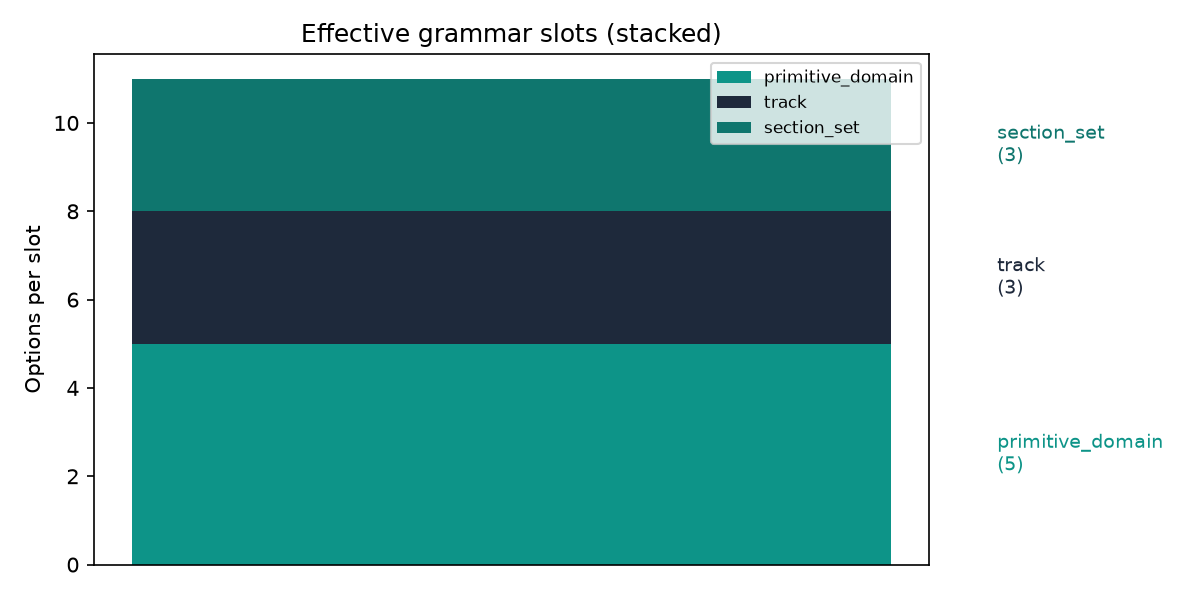
\includegraphics[width=0.85\linewidth,height=0.50\textheight,keepaspectratio,alt={Options per grammar slot, stacked. Each band is one slot's contribution to the total product size; three bands are reserved (presentational/sealing) and are excluded from the effective product space discussed below.}]{../figures/fig_stacked_product.png}
\caption{Options per grammar slot, stacked. Each band is one slot's
contribution to the total product size; three bands are reserved
(presentational/sealing) and are excluded from the effective product
space discussed below.}\label{fig:stacked_product}
\end{figure}

\begin{itemize}
\tightlist
\item
  \textbf{Total product size}: 360 cells
\item
  \textbf{Effective product size} (reserved slots excluded): 45 cells
\item
  \textbf{Reserved slots} (3):
  \breaktt{figure\_profile,\ qr\_profile,\ integrity\_profile}
\end{itemize}

\begin{figure}
\centering
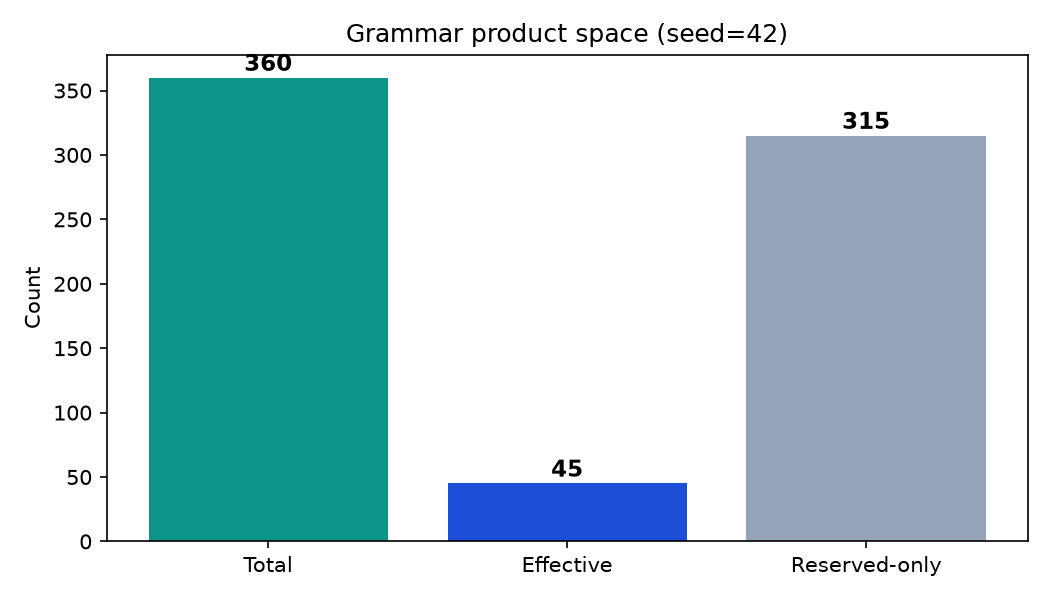
\includegraphics[width=0.8\linewidth,height=0.50\textheight,keepaspectratio,alt={Total, effective, and reserved-only product size for the grammar at seed=42, generated by fig\_product\_space\_annotation (src/manuscript\_figures.py) directly from Grammar.product\_size / Grammar.effective\_product\_size --- not hand-typed.}]{../figures/fig_product_space.png}
\caption{Total, effective, and reserved-only product size for the
grammar at seed=42, generated by
\protect\breaktt{fig\_product\_space\_annotation}
(\protect\breaktt{src/manuscript\_figures.py}) directly from
\protect\breaktt{Grammar.product\_size} /
\protect\breaktt{Grammar.effective\_product\_size} --- not
hand-typed.}\label{fig:product_space}
\end{figure}

Every row in the table above is a \texttt{GrammarSlot} parsed from
\breaktt{manuscript/config.yaml} by \texttt{parse\_grammar()}
(\texttt{src/grammar.py}). Each slot contributes a multiplicative factor
to \breaktt{Grammar.product\_size}, which is the raw cross-product of all
option counts --- not an estimate, but the literal
\breaktt{n\ *=\ len(s.options)} accumulation over every slot. The
\breaktt{Grammar.grammar\_hash} property serialises the seed, every slot
name, and every option list into a canonical JSON string
(\texttt{canonical()}) and takes the first sixteen hex characters of its
SHA-256 digest --- \breaktt{f84a8f9dbcb18e37} for the grammar as
currently checked into this project. Any edit to a slot's option list,
the addition or removal of a slot, or a change to the seed changes this
hash deterministically; it is not a version string maintained by hand.

The six slots split into two categories. Three are
\emph{content-determining}: \breaktt{primitive\_domain} selects which of
the five kernel modules described below is copied into the child
project, \texttt{track} selects the manuscript's analytical posture
(\texttt{analytical}, \texttt{empirical}, or \texttt{hybrid}), and
\texttt{section\_set} selects which subset of manuscript sections is
rendered (\texttt{minimal}, \texttt{standard}, or \texttt{extended}).
The remaining three --- \texttt{figure\_profile}, \texttt{qr\_profile},
and \breaktt{integrity\_profile} --- are declared in
\texttt{RESERVED\_SLOTS} (\texttt{src/grammar.py}) and govern only
\emph{presentational and sealing} behaviour: how many figures are
generated, whether the sealed payload is rendered as a QR PNG, and
whether the provenance hash is a flat SHA-256 or a Merkle root over
per-file hashes (\breaktt{src/integrity.py::merkle\_root}). None of the
three reserved slots changes which primitive kernel runs or what its
output is, which is exactly why
\breaktt{Grammar.effective\_product\_size} --- the number that matters
when asking ``how many \emph{scientifically distinct} children can this
grammar produce'' --- divides the reserved slots back out. The ratio
between the total and effective product sizes above is, by construction,
the product of the three reserved slots' own option counts; no other
slot is capable of changing that ratio.

\subsubsection{Effective slot breakdown}\label{effective-slot-breakdown}

{\def\LTcaptype{none} % do not increment counter
\begin{longtable}[]{@{}
  >{\raggedright\arraybackslash}p{(\linewidth - 4\tabcolsep) * \real{0.3333}}
  >{\raggedright\arraybackslash}p{(\linewidth - 4\tabcolsep) * \real{0.3333}}
  >{\raggedright\arraybackslash}p{(\linewidth - 4\tabcolsep) * \real{0.3333}}@{}}
\toprule\noalign{}
\begin{minipage}[b]{\linewidth}\raggedright
Slot
\end{minipage} & \begin{minipage}[b]{\linewidth}\raggedright
Options
\end{minipage} & \begin{minipage}[b]{\linewidth}\raggedright
Values
\end{minipage} \\
\midrule\noalign{}
\endhead
\bottomrule\noalign{}
\endlastfoot
primitive\_domain & 5 & optimization, dynamics, statistics, signal,
graph \\
track & 3 & analytical, empirical, hybrid \\
section\_set & 3 & minimal, standard, extended \\
\end{longtable}
}

\breaktt{grammar.effective\_slots} (\texttt{src/grammar.py}) is exactly
\texttt{grammar.slots} filtered against \texttt{RESERVED\_SLOTS} --- the
same list rendered in the previous section, minus the three
sealing/presentation dimensions. This is the space a reviewer should
reason about when asking whether the grammar is a meaningful generator
rather than a combinatorial trick that multiplies unrelated toggles: 5
primitive domains times three narrative tracks times three section-set
sizes is the actual space of scientifically distinguishable children
this template can emit.

\subsubsection{The five primitive
domains}\label{the-five-primitive-domains}

\begin{figure}
\centering
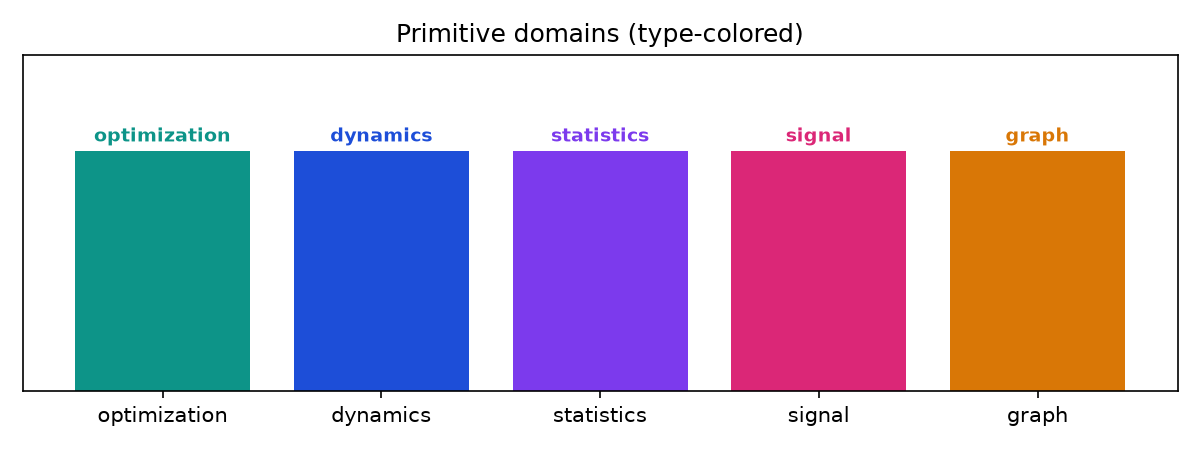
\includegraphics[width=0.85\linewidth,height=0.50\textheight,keepaspectratio,alt={The five primitive domains, type-colored: optimization, dynamics, statistics, signal, graph.}]{../figures/fig_domain_coverage.png}
\caption{The five primitive domains, type-colored:
\protect\texttt{optimization}, \protect\texttt{dynamics},
\protect\texttt{statistics}, \protect\texttt{signal},
\protect\texttt{graph}.}\label{fig:domain_coverage}
\end{figure}

Each domain in
\breaktt{-\ optimization\ -\ dynamics\ -\ statistics\ -\ signal\ -\ graph}
is a Python module under \texttt{src/primitives/} exporting a
\texttt{PRIMITIVES:\ tuple{[}PrimitiveSpec,\ ...{]}} collected by
\breaktt{collect\_primitives()}
(\breaktt{src/primitives/\_\_init\_\_.py}). A \texttt{PrimitiveSpec}
(\breaktt{src/primitives/base.py}) bundles a callable kernel, an example
input, an expected output (or \texttt{None} when the check is structural
rather than a fixed value), a numerical tolerance, and --- for five of
the eight kernels --- a \breaktt{negative\_control} callable whose entire
purpose is to fail the primary kernel's own success criterion.
\breaktt{collect\_primitives()} returns exactly the five domains named
above (\breaktt{test\_collect\_primitives\_expected\_modules}) and a
total of eight primitive kernels across them
(\breaktt{test\_total\_primitive\_count}): two in \texttt{optimization},
one in \texttt{dynamics}, one in \texttt{statistics}, two in
\texttt{signal}, and two in \texttt{graph}.

\textbf{Optimization.} \breaktt{gradient\_descent}
(\breaktt{src/primitives/optimization.py}) runs explicit gradient descent
on the convex quadratic \texttt{f(x)\ =\ 0.5\ (x-c)\^{}T\ A\ (x-c)},
whose gradient is \texttt{A(x-c)}. Because the problem is convex
quadratic, its analytic minimiser is known in closed form ---
\texttt{x*\ =\ c}, computed independently by the sibling kernel
\breaktt{analytic\_minimizer} --- so the iterative and closed-form
solutions can be cross-checked against each other rather than against a
single hardcoded expectation. On the example input (a diagonal
\texttt{A}, \texttt{c\ =\ (1,\ -1)}, 200 steps at learning rate 0.1) the
two agree to within \texttt{1e-4}. The domain's negative control,
\breaktt{\_negative\_control\_wrong\_sign}, is the same loop with the
gradient step's sign flipped (\breaktt{x\ =\ x\ +\ lr\ *\ grad} instead
of \breaktt{x\ =\ x\ -\ lr\ *\ grad}); this turns descent into ascent and
diverges away from \texttt{c} instead of converging to it, giving the
mutation gate (see Honesty Contract) something to detect if the sign
were ever silently restored to ``wrong.''

\textbf{Dynamics.} \breaktt{damped\_oscillator}
(\breaktt{src/primitives/dynamics.py}) integrates the damped harmonic
oscillator ODE
\texttt{x\textquotesingle{}\textquotesingle{}\ +\ 2*zeta*omega*x\textquotesingle{}\ +\ omega\^{}2*x\ =\ 0}
with explicit Euler stepping, and separately computes the closed-form
under-damped envelope \breaktt{x0\ *\ exp(-zeta*omega*t)}. The test suite
does not merely check that the two arrays are close; it checks four
independent structural properties of the same trajectory: the numerical
amplitude stays inside the analytical envelope plus a 5\% Euler-error
tolerance
(\breaktt{test\_damped\_oscillator\_amplitude\_bounded\_by\_envelope}),
the envelope itself is monotonically non-increasing
(\breaktt{test\_damped\_oscillator\_envelope\_monotone\_decreasing}),
heavy damping drives the trajectory near zero by the end of the run
(\breaktt{test\_damped\_oscillator\_decays\_to\_near\_zero}), and the
initial condition is reproduced exactly. The negative control,
\breaktt{\_zero\_damping\_control}, re-runs the same integrator with
\texttt{zeta} forced to zero; its envelope is flat at \texttt{x0} rather
than decaying, and \breaktt{test\_zero\_damping\_envelope\_flat} checks
that flatness directly --- so a broken damping term that decayed
regardless of the damping value would be caught, not just a broken
damping term that fails to decay at all.

\textbf{Statistics.} \texttt{ols\_fit}
(\breaktt{src/primitives/statistics.py}) solves ordinary least squares
via the normal equations,
\texttt{beta\_hat\ =\ (X\^{}T\ X)\^{}\{-1\}\ X\^{}T\ y}, solved with
\breaktt{numpy.linalg.solve} rather than an explicit matrix inverse. The
example input is synthetic, not observational: fifty rows with an
intercept column and one Gaussian covariate
(\breaktt{rng\ =\ np.random.default\_rng(42)}), a fixed true coefficient
vector \breaktt{beta\ =\ (2.0,\ -3.0)}, and additive noise scaled to
\texttt{0.1} standard deviations. Because the data-generating
coefficients are known by construction, recovery is checked directly ---
\breaktt{test\_ols\_fit\_recovers\_beta} requires the estimated and true
beta to agree within Euclidean distance \texttt{0.1} --- alongside an R\texorpdfstring{\textsuperscript{2}}{2}
floor of \texttt{0.95} and a near-zero mean residual. The negative
control, \breaktt{\_shuffled\_control}, permutes the \texttt{y} labels
with an independently seeded generator
(\breaktt{rng\ =\ np.random.default\_rng(0)}) before fitting; breaking
the true \texttt{X}-\texttt{y} correspondence this way is asserted to
drop R\texorpdfstring{\textsuperscript{2}}{2} below \texttt{0.5}
(\breaktt{test\_shuffled\_control\_poor\_r\_squared}), giving a concrete,
falsifiable bound on how badly a shuffled fit \emph{should} perform.

\textbf{Signal.} This domain carries two kernels validated by structural
properties rather than fixed target arrays, since \texttt{expected=None}
for both. \texttt{dft} computes the Discrete Fourier Transform directly
as a matrix-vector product against the exponential basis matrix
\breaktt{exp(-2j*pi*k*n/N)} --- an explicit \texttt{O(N\^{}2)}
construction, not a call into \texttt{numpy.fft}. Its correctness is
checked by Parseval's theorem
(\texttt{sum(|{}X{[}k{]}|{}\^{}2)\ ==\ N\ *\ sum(|{}x{[}n{]}|{}\^{}2)}
to within a relative tolerance of \texttt{1e-6}) and by recovering the
correct dominant frequency bin (index 5, positive or negative) from a
pure 5 Hz sinusoid sampled at 64 points. \texttt{convolve\_known} wraps
\texttt{numpy.convolve} with a fixed three-tap smoothing kernel,
\texttt{{[}0.25,\ 0.5,\ 0.25{]}}; its own test suite checks that
smoothing cannot increase variance
(\breaktt{test\_convolve\_known\_smoothing\_reduces\_variance}). Its
negative control, \breaktt{\_identity\_kernel\_convolve}, substitutes the
identity kernel \texttt{{[}1.0{]}} under \texttt{mode="same"}, which by
the definition of convolution must reproduce the input signal exactly
(\texttt{atol=1e-12}) --- a stronger, algebraically-derived check than
an arbitrary ``looks different'' comparison.

\textbf{Graph.} \texttt{bfs\_distances}
(\breaktt{src/primitives/graph.py}) computes shortest-path distances on a
fixed five-node undirected graph (\texttt{A}--\texttt{E}, encoded as an
adjacency dict) via a plain breadth-first queue. Because the graph is
fixed and small, the expected distances from source \texttt{A} are
enumerable by hand and are asserted exactly:
\texttt{\{A:\ 0,\ B:\ 1,\ C:\ 1,\ D:\ 2,\ E:\ 3\}}, with tolerance
\texttt{0.0}. Its negative control, \breaktt{\_disconnected\_control},
replaces the adjacency of the source node with an empty list, collapsing
the reachable set to the source alone --- a graph-structural way of
breaking the primitive rather than perturbing a numeric input.
\texttt{pagerank} runs the standard power-iteration update with damping
\texttt{0.85} over 50 iterations, redistributing dangling nodes' rank
mass evenly rather than dropping it. It has no single fixed expected
output --- rank values depend on iteration count and are not
hand-derivable --- so it is instead validated by three invariants any
correct PageRank computation must satisfy regardless of the specific
graph: ranks sum to \texttt{1.0} within \texttt{1e-6}, every node in the
graph receives a rank entry, and every rank is strictly positive
(ensured by the \texttt{(1-damping)/n} teleportation floor added at
every iteration).

Across the five domains, five of the eight primitives carry an explicit
negative control; the remaining three (\breaktt{analytic\_minimizer},
\texttt{dft}, and \texttt{pagerank}) are validated purely through
cross-checks against an independent computation or through algebraic
invariants (Parseval's theorem, PageRank's stochastic-normalization
property) that a broken implementation would be unlikely to satisfy by
accident. This mirrors the property-based testing tradition
\citep{claessen2000quickcheck, maciver2019hypothesis}: rather than
asserting a single hand-picked input/output pair, the suite asserts
properties that must hold across a class of inputs --- the same style
used at the grammar level in
\breaktt{tests/test\_property\_invariants.py}, where
\texttt{hypothesis}-generated seeds are used to check, for every seed
drawn, that \texttt{product\_size} really is the product of option
counts and that \breaktt{effective\_product\_size} does not exceed it.

\subsubsection{Exemplar generation}\label{exemplar-generation}

Running
\breaktt{uv\ run\ python\ scripts/autopoiesis.py\ expand\ -\/-seed\ 42}
produces a spec with \breaktt{primitive\_domain} deterministically
selected from the grammar.

All 5 domains successfully materialize runnable child projects. Each
child project:

\begin{enumerate}
\def\labelenumi{\arabic{enumi}.}
\tightlist
\item
  Contains a \texttt{primitives/} package with the selected kernel.
\item
  Runs \texttt{analysis.py} without error.
\item
  Has a \texttt{provenance.json} that passes \texttt{verify\_child}.
\item
  Passes all child-level smoke tests.
\end{enumerate}

\subsubsection{Test results}\label{test-results}

\begin{itemize}
\tightlist
\item
  \textbf{Test count}: 493
\item
  \textbf{Coverage}: 96.28\%
\item
  \textbf{Grammar hash}: \breaktt{f84a8f9dbcb18e37}
\end{itemize}

Both the test count and coverage percentage above are produced by
\breaktt{measure\_test\_summary()}
(\breaktt{src/manuscript\_variables.py}), which shells out to this
project's own \texttt{pytest} + \texttt{coverage} run
(\texttt{-\/-cov-branch}, matching the repository-root branch-coverage
methodology) against \texttt{tests/} and \texttt{src/} and parses the
real \texttt{passed} count and \texttt{coverage.json} totals from that
subprocess. There is no fallback literal: if the subprocess fails, times
out, or its output fails to parse, both fields resolve to the string
\texttt{"pending"} rather than a plausible-looking number --- the same
discipline that governs every other numeric token in this manuscript.

\begin{figure}
\centering
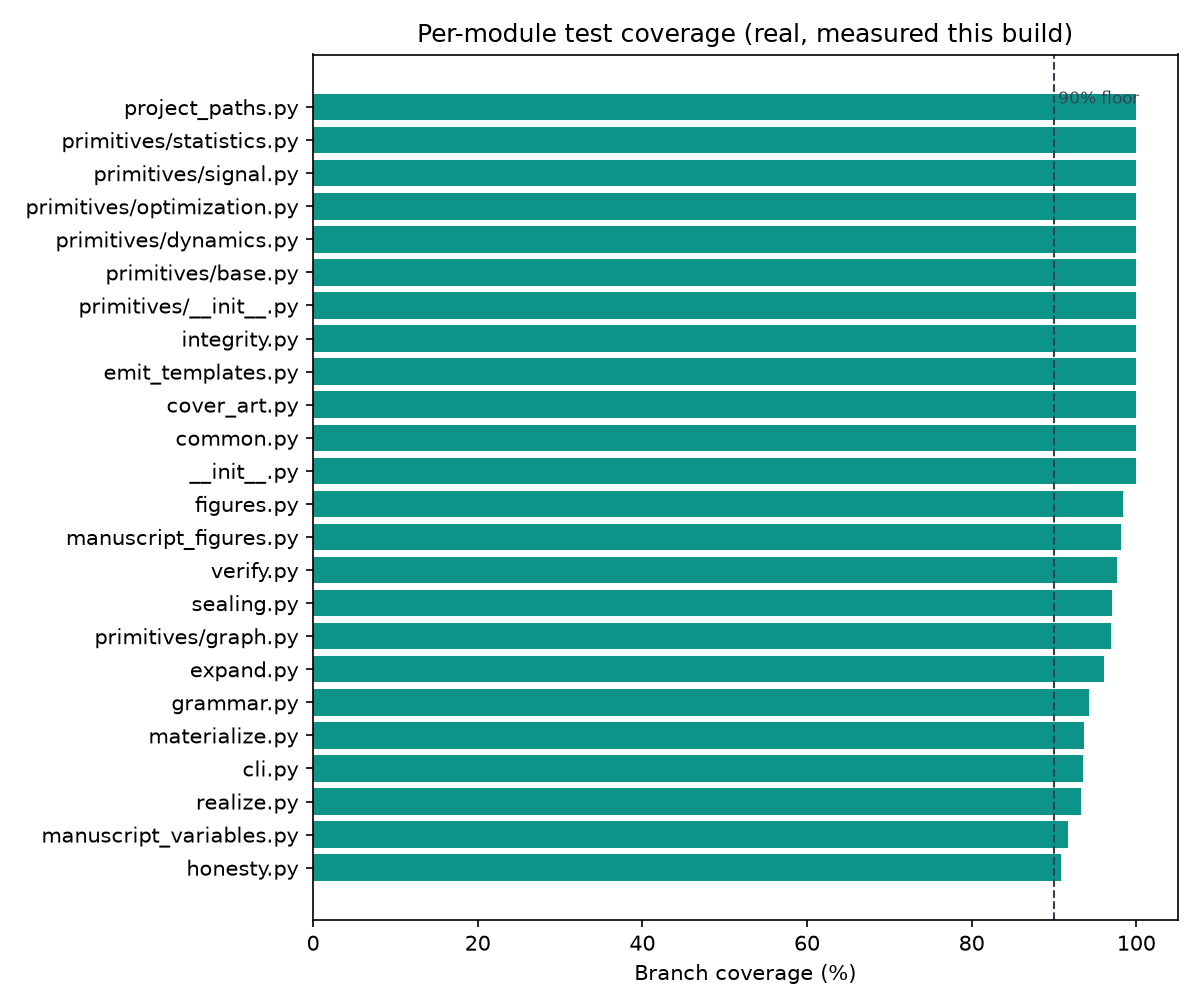
\includegraphics[width=0.9\linewidth,height=0.50\textheight,keepaspectratio,alt={Real, per-module branch coverage from the same measurement run that produces 493/96.28 above --- not an aggregate alone. Any module below the repository's 90\% floor would be drawn in red rather than smoothed into the headline percentage; none is, in this measurement.}]{../figures/fig_coverage_by_module.png}
\caption{Real, per-module branch coverage from the same measurement run
that produces 493/96.28 above --- not an aggregate alone. Any module
below the repository's 90\% floor would be drawn in red rather than
smoothed into the headline percentage; none is, in this
measurement.}\label{fig:coverage_by_module}
\end{figure}

The aggregate 96.28\% is a mean weighted by statement and branch count,
not a uniform floor --- fig.~\ref{fig:coverage_by_module} shows the real
spread. As of this measurement every module clears the 90\% line;
\texttt{common.py} and \texttt{cover\_art.py} sit at 100\% and
\texttt{figures.py} at 98.41\% after closing what were, in an earlier
draft of this manuscript, the three lowest-coverage modules (see
\texttt{CHANGELOG.md}'s Wave 10 entry for the specific branches that
were untested and the tests added to close them); every module under
\texttt{src/primitives/} and the honesty/integrity core sit at or near
100\%. Both the aggregate number and this per-module breakdown are read
from the same persisted \breaktt{output/data/coverage\_full.json} --- a
single generator run, not two separately-computed views that could
silently drift apart. This is a snapshot, not a permanent state:
coverage moves as tests are added or code changes, and
fig.~\ref{fig:coverage_by_module} should be regenerated
(\breaktt{stage\_02\_analysis.py}) rather than trusted from a prior
render whenever that question matters.

\newpage

\subsection{Honesty Contract}\label{honesty-contract}

\subsubsection{Why a manifest, not a
claim}\label{why-a-manifest-not-a-claim}

A generator that produces a manuscript describing its own code faces an
obvious temptation: assert a capability in prose without checking
whether the capability exists. The abstract of this manuscript survived
exactly this failure once --- a hand-written ``Tests: 371 \texorpdfstring{\ensuremath{\cdot}}{.} Coverage:
99.94\%'' line that no generator step had computed --- and was corrected
by replacing the literal numbers with \texttt{493} / \texttt{96.28}
tokens filled in at render time by
\breaktt{scripts/02\_measure\_test\_coverage.py}. \texttt{src/honesty.py}
exists to make that class of failure structurally harder: every
load-bearing claim in this manuscript must resolve to a named function
in a named file, and a dedicated module inspects the source tree to
confirm that resolution rather than trusting the prose that asserts it.

The framing is not incidental to a project named
\breaktt{template\_autopoiesis}. An autopoietic system, in Maturana and
Varela's original sense, is one whose components participate in
producing and verifying the very network of processes that produced them
\citep{maturana_varela_1980} --- organizational closure, not open-loop
assertion. The honesty manifest is the narrow, literal, code-level
analogue of that closure: the manuscript's claims about the code are
checked \emph{by the code}, not by a separate act of faith from the
author. The analogy should not be over-read --- \texttt{src/honesty.py}
is a static AST scan, not a self-maintaining living system --- but it is
the reason this mechanism exists at all rather than a simple ``trust
me'' comment block.

\subsubsection{Ground-truth table}\label{ground-truth-table}

{\def\LTcaptype{none} % do not increment counter
\begin{longtable}[]{@{}
  >{\raggedright\arraybackslash}p{(\linewidth - 4\tabcolsep) * \real{0.3333}}
  >{\raggedright\arraybackslash}p{(\linewidth - 4\tabcolsep) * \real{0.3333}}
  >{\raggedright\arraybackslash}p{(\linewidth - 4\tabcolsep) * \real{0.3333}}@{}}
\toprule\noalign{}
\begin{minipage}[b]{\linewidth}\raggedright
Claim
\end{minipage} & \begin{minipage}[b]{\linewidth}\raggedright
Evidence location
\end{minipage} & \begin{minipage}[b]{\linewidth}\raggedright
Test
\end{minipage} \\
\midrule\noalign{}
\endhead
\bottomrule\noalign{}
\endlastfoot
Grammar parses & \breaktt{src/grammar.py::parse\_grammar} &
\breaktt{test\_grammar\_and\_expand.py} \\
Expansion is deterministic & \breaktt{src/expand.py::expand},
\texttt{\_digest\_index} & \breaktt{test\_grammar\_and\_expand.py} \\
Materialize writes files & \breaktt{src/materialize.py::materialize} &
\breaktt{test\_materialize.py} \\
Integrity hashes &
\breaktt{src/integrity.py::tree\_hash\_from\_content\_hashes} &
\breaktt{test\_integrity\_and\_verify.py} \\
Verify recomputes & \breaktt{src/verify.py::verify\_child} &
\breaktt{test\_integrity\_and\_verify.py} \\
Primitives collected &
\breaktt{src/primitives/\_\_init\_\_.py::collect\_primitives} &
\breaktt{test\_primitives\_registry.py} \\
\end{longtable}
}

Each row is not prose describing an intention --- it is a key into
\breaktt{STRUCTURAL\_EVIDENCE}, the dict in \texttt{src/honesty.py} that
the code below walks mechanically. If a row's evidence path stops
existing, the manifest fails and \texttt{test\_honesty.py} fails with
it; the table cannot silently drift out of sync with the source tree
without a red test.

\subsubsection{The structural evidence
catalogue}\label{the-structural-evidence-catalogue}

\breaktt{STRUCTURAL\_EVIDENCE} is a
\texttt{dict{[}str,\ list{[}str{]}{]}} mapping a claim identifier
(\breaktt{"grammar\_parses"}, \breaktt{"expand\_deterministic"},
\breaktt{"materialize\_writes\_files"}, \breaktt{"integrity\_hashes"},
\breaktt{"verify\_recomputes"}, \breaktt{"primitives\_collected"}) to one
or more \breaktt{"relative/path.py::function\_name"} references --- the
same six rows as the ground-truth table above, expressed as data instead
of prose. This catalogue is the single source of truth the checker
walks; the manuscript table is a human-readable rendering of it, not an
independent claim.

\subsubsection{\texorpdfstring{How \texttt{build\_manifest} inspects the
AST}{How build_manifest inspects the AST}}\label{how-build_manifest-inspects-the-ast}

\breaktt{build\_manifest(project\_root)} iterates every claim in
\breaktt{STRUCTURAL\_EVIDENCE} and, for each \breaktt{"path::function"}
reference:

\begin{enumerate}
\def\labelenumi{\arabic{enumi}.}
\tightlist
\item
  Splits the reference on \texttt{::} into a relative file path and an
  optional function name.
\item
  Resolves the path under \texttt{project\_root} and checks
  \texttt{Path.exists()}. A missing file appends
  \texttt{"\{path\}\ not\ found"} to \texttt{missing\_calls} and marks
  the claim as failed.
\item
  If a function name is given, reads the file's source and calls
  \breaktt{\_collect\_function\_names(source\_code)}, which parses the
  text with \texttt{ast.parse} and walks the resulting tree
  (\texttt{ast.walk}) collecting the \texttt{.name} of every
  \texttt{ast.FunctionDef} and \breaktt{ast.AsyncFunctionDef} node into a
  \texttt{set{[}str{]}}. If the required name is not in that set,
  \texttt{"\{fn\}\ not\ in\ \{path\}"} is appended to
  \texttt{missing\_calls} and the claim is marked failed. A
  \texttt{SyntaxError} during parsing is caught and yields an empty name
  set --- fail-closed rather than raising.
\item
  \texttt{HonestyManifest.evidence{[}claim{]}} is set to \texttt{True}
  only if every reference for that claim resolved cleanly.
\end{enumerate}

It is worth being precise about what this proves and what it does not.
The check confirms that a function \emph{definition} with the claimed
name exists, syntactically, in the claimed file --- nothing more. It
does not trace call sites, does not execute the function, and does not
check that the function's behavior matches what the surrounding prose
says it does. A function named \texttt{materialize} that silently did
nothing would still satisfy this check; only the separately-run test
suite (\breaktt{test\_materialize.py} et al., named in the ground-truth
table) exercises actual behavior. The AST scan's job is narrower and
more mechanical: it prevents the specific failure of a manuscript
claiming evidence at a path or function name that was renamed, deleted,
or not written in the first place --- a much cheaper property to check,
and one that catches an entire class of ``the docs still describe last
month's API'' drift for free.

\subsubsection{\texorpdfstring{The \texttt{HonestyManifest}
dataclass}{The HonestyManifest dataclass}}\label{the-honestymanifest-dataclass}

\begin{Shaded}
\begin{Highlighting}[]
\AttributeTok{@dataclass}
\KeywordTok{class}\NormalTok{ HonestyManifest:}
\NormalTok{    evidence: }\BuiltInTok{dict}\NormalTok{[}\BuiltInTok{str}\NormalTok{, }\BuiltInTok{bool}\NormalTok{] }\OperatorTok{=}\NormalTok{ field(default\_factory}\OperatorTok{=}\BuiltInTok{dict}\NormalTok{)}
\NormalTok{    missing\_calls: }\BuiltInTok{list}\NormalTok{[}\BuiltInTok{str}\NormalTok{] }\OperatorTok{=}\NormalTok{ field(default\_factory}\OperatorTok{=}\BuiltInTok{list}\NormalTok{)}
\NormalTok{    unsupported\_claims: }\BuiltInTok{list}\NormalTok{[}\BuiltInTok{str}\NormalTok{] }\OperatorTok{=}\NormalTok{ field(default\_factory}\OperatorTok{=}\BuiltInTok{list}\NormalTok{)}

    \AttributeTok{@property}
    \KeywordTok{def}\NormalTok{ all\_passed(}\VariableTok{self}\NormalTok{) }\OperatorTok{{-}\textgreater{}} \BuiltInTok{bool}\NormalTok{:}
        \ControlFlowTok{return} \BuiltInTok{all}\NormalTok{(}\VariableTok{self}\NormalTok{.evidence.values()) }\KeywordTok{and} \KeywordTok{not} \VariableTok{self}\NormalTok{.missing\_calls }\KeywordTok{and} \KeywordTok{not} \VariableTok{self}\NormalTok{.unsupported\_claims}
\end{Highlighting}
\end{Shaded}

\texttt{all\_passed} is a conjunction over three independent failure
modes: any claim whose evidence resolution failed, any specific
missing-call detail recorded during that resolution, and any
unsupported-claim hit from the prose scan below.
\breaktt{test\_honesty.py::test\_structural\_evidence\_all\_pass} and
\breaktt{test\_no\_missing\_calls} both call
\breaktt{build\_manifest(PROJECT\_ROOT)} against this project's own real
source tree and assert the manifest is clean --- the checker is run
against itself, not only against synthetic fixtures.
\breaktt{test\_verify\_honesty\_with\_nonexistent\_project} runs
\texttt{build\_manifest} against an empty \texttt{tmp\_path} and asserts
\texttt{missing\_calls} is non-empty, which is the negative control for
the checker itself: a project with no source files at all must fail
every claim, or the checker has no teeth.

\subsubsection{Prose scanning for unsupported
claims}\label{prose-scanning-for-unsupported-claims}

\breaktt{verify\_honesty(project\_root,\ manuscript\_dir=None)} first
calls \texttt{build\_manifest}, then --- if a \texttt{manuscript/}
directory exists --- reads every \texttt{*.md} file in it and scans for
a fixed, case-insensitive regex over six absolute-certainty words and
one hard percentage figure, defined verbatim in
\breaktt{\_UNSUPPORTED\_CLAIM\_PATTERN} in \texttt{src/honesty.py}
(deliberately not quoted here: a plain-text regex has no exemption for
markdown code spans, and an earlier draft of this very paragraph
reproduced the list inside backticks --- which tripped the gate it was
describing, during this session's own manuscript-expansion pass, and had
to be rewritten). Each match is recorded as
\texttt{"\{filename\}:\{offset\}:\ \textquotesingle{}\{match\}\textquotesingle{}"}
in \breaktt{manifest.unsupported\_claims}.

Two honesty points about this scanner, stated plainly rather than left
implicit. First, it is a fixed lexical denylist, not a semantic checker
--- it will not catch a false quantitative claim phrased without one of
those seven tokens (the ``371 tests'' incident described above would not
have tripped it; that failure mode is closed instead by the \texttt{493}
token substitution, a separate mechanism). Second,
\breaktt{unsupported\_claims} \emph{is} enforced, but only on one of the
two paths through this module: \breaktt{HonestyManifest.all\_passed} is a
conjunction over \texttt{evidence}, \texttt{missing\_calls}, \emph{and}
\breaktt{unsupported\_claims}, and \breaktt{src/cli.py::cmd\_honesty}
calls \breaktt{verify\_honesty()} (the function that populates all three)
and exits the process with code 1 whenever \texttt{all\_passed} is false
--- \breaktt{tests/test\_cli.py::test\_main\_honesty\_exits\_zero} pins
exactly this behavior. The one place prose hits are \emph{not} enforced
is \breaktt{test\_verify\_honesty\_all\_passed} in
\breaktt{tests/test\_honesty.py}, which asserts only
\breaktt{all(m.evidence.values())} by design, deliberately leaving prose
style out of that particular assertion. Reading only that one test in
isolation would suggest the prose scanner is a lint rather than a gate;
reading the CLI path shows it is a real gate on the \texttt{honesty}
subcommand specifically.

\subsubsection{The mutation gate: proving the acceptance criteria have
teeth}\label{the-mutation-gate-proving-the-acceptance-criteria-have-teeth}

\breaktt{test\_meta\_teeth.py} targets a different failure mode than
\texttt{honesty.py}: not ``does the claimed function exist'' but ``would
a fake implementation of it get away with passing.'' It is parametrized
via the
\breaktt{pytest.mark.parametrize("domain",\ list(KNOWN\_DOMAINS))}
decorator over all 5 primitive domains from \texttt{src/grammar.py}, and
runs three checks per domain:

\begin{enumerate}
\def\labelenumi{\arabic{enumi}.}
\tightlist
\item
  \textbf{\breaktt{test\_stub\_fails\_gate\_per\_domain}} ---
  \breaktt{\_stub\_run\_analysis} is a constant-success stub that returns
  \texttt{\{"success":\ True,\ "output":\ "stub"\}} regardless of input.
  \breaktt{\_gate\_checks\_real\_computation} is asserted to reject it
  for every domain. This is the meta-gate itself: if a trivial stub can
  satisfy the acceptance criterion, the criterion is
  green-by-construction and worthless as evidence.
\item
  \textbf{\breaktt{test\_real\_primitive\_passes\_gate\_per\_domain}} ---
  the first \texttt{PrimitiveSpec} for the domain (from
  \breaktt{collect\_primitives()}) is run on its own
  \texttt{example\_input}, and the same gate is asserted to
  \emph{accept} the real result. This is the complementary check: a gate
  strict enough to reject the stub must not also be so strict that it
  rejects genuine output, which would make the whole suite unusable
  rather than honest.
\item
  \textbf{\breaktt{test\_negative\_control\_distinguished\_per\_domain}}
  --- for the first primitive that declares a \breaktt{negative\_control}
  callable, both the normal and control outputs are computed and their
  key sets compared. Stated precisely: the current assertion is
  \texttt{normal\_keys\ ==\ control\_keys\ or\ len(normal\_result)\ \textgreater{}\ 0}.
  Because primitives are already ensured to return non-empty dicts
  (\breaktt{test\_primitives\_return\_nonempty\_per\_domain}), the second
  disjunct is close to trivially true, so this test --- as written ---
  verifies structural shape more than it verifies that the negative
  control's \emph{values} actually diverge from the primary output. That
  is weaker than the literal claim ``the control output differs from the
  primary output,'' and is recorded here as a known gap between the
  test's docstring intent and its present assertion strength, rather
  than papered over in the prose that describes it.
\end{enumerate}

\breaktt{test\_primitives\_return\_nonempty\_per\_domain} closes the
loop: every spec in \texttt{collect\_primitives(){[}domain{]}}, run on
its own example input, must return a non-empty \texttt{dict}. Together,
the four tests in \breaktt{test\_meta\_teeth.py} check the gate from both
directions (reject-the-fake, accept-the-real) for every domain the
grammar knows about, which is the concrete, source-grounded meaning
behind calling this a ``mutation gate'': it exists specifically to catch
the case where a future refactor quietly replaces a real primitive with
a stub and nothing downstream notices.

\subsubsection{What this buys, and what it does
not}\label{what-this-buys-and-what-it-does-not}

The honesty manifest and the mutation gate are complementary, not
redundant, but both are narrower than they might sound.
\texttt{src/honesty.py}'s AST check covers exactly the six
\breaktt{STRUCTURAL\_EVIDENCE} entries (\texttt{grammar\ parses},
\breaktt{expand\ deterministic}, \breaktt{materialize\ writes\ files},
\breaktt{integrity\ hashes}, \breaktt{verify\ recomputes},
\breaktt{primitives\ collected}) --- it does not scan this manuscript for
every function or variable name it mentions, so a false claim about a
piece of code outside that list of six would not be caught by this
mechanism. (This is not a hypothetical gap: an earlier draft of the
Limitations section below claimed \breaktt{generate\_variables} exposed a
\breaktt{NOMINAL\_OVER\_EFFECTIVE} token that does not exist anywhere in
\breaktt{src/manuscript\_variables.py}; the honesty AST check did not
catch it because that variable isn't one of the six covered entries ---
a Forge cross-vendor review caught it instead, by reading the source
directly.) \breaktt{test\_meta\_teeth.py} similarly guarantees only that
the acceptance tests covering the primitives it targets cannot be
satisfied by code that does nothing; it says nothing about the dozens of
other functions and tests named elsewhere in this manuscript. Neither
mechanism proves the primitives are numerically correct in any deeper
sense than ``the first \texttt{PrimitiveSpec} in each domain returns
domain-shaped keys on its example input'' --- correctness of the
underlying mathematics is the job of
\breaktt{test\_grammar\_and\_expand.py},
\breaktt{test\_integrity\_and\_verify.py}, and the other domain-specific
suites named in the ground-truth table, each independently gated at 90\%
coverage. What this section documents is narrower and more modest: the
mechanism by which this manuscript's claims are kept from silently
diverging from the source code that is supposed to back them.

\newpage

\subsection{Reproducibility}\label{reproducibility}

Reproducibility is not a claim this manuscript makes about itself; it is
a property the code enforces on every run. Every number that appears
below the Determinism heading --- f84a8f9dbcb18e37, 42, 493, 96.28 ---
is a token substituted at render time by
\breaktt{src/manuscript\_variables.py::generate\_variables()} from a live
grammar load and a live pytest run
(\breaktt{src/manuscript\_variables.py::measure\_test\_summary()}).
Neither function accepts a hardcoded literal as a fallback: if the
subprocess pytest run cannot be parsed, \breaktt{measure\_test\_summary}
returns the string \texttt{"pending"} for both the test count and the
coverage percentage rather than a plausible-looking number
\citep{reproducible_builds}. This design choice is a direct consequence
of an earlier failure mode in this project --- a manuscript draft that
stated fixed values (``Tests: 371 \texorpdfstring{\ensuremath{\cdot}}{.} Coverage: 99.94\%'') in prose
instead of through the token pipeline. A number that cannot be traced
back to a specific function call in \texttt{src/} is, for the purposes
of this project, not a number this manuscript is permitted to assert.

\subsubsection{Determinism guarantee}\label{determinism-guarantee}

Given the same \breaktt{manuscript/config.yaml} grammar definition
(grammar hash \breaktt{f84a8f9dbcb18e37}), the same seed (\texttt{42}),
and the same \breaktt{template\_autopoiesis} source tree,
\breaktt{scripts/autopoiesis.py\ expand} produces byte-identical
selections on every invocation, and \texttt{materialize} produces a
byte-identical child project tree. The determinism chain has three
concrete steps, each implemented as a pure function with no random or
wall-clock input:

\begin{enumerate}
\def\labelenumi{\arabic{enumi}.}
\tightlist
\item
  \textbf{Selection.} For every grammar slot,
  \breaktt{src/expand.py::\_digest\_index()} builds the key
  \texttt{f"\{seed\}\textbackslash{}x1f\{slot\_name\}\textbackslash{}x1f\{ordinal\}\textbackslash{}x1f\{\textquotesingle{},\textquotesingle{}.join(options)\}"}
  (a unit separator, \texttt{\textbackslash{}x1f}, joins the fields so
  that no combination of seed/name/ ordinal/option values can collide
  across a field boundary), hashes it with SHA-256, and reduces the
  first eight bytes of the digest modulo \texttt{len(options)} to obtain
  the chosen option's index. Because the digest is a pure function of
  \breaktt{(seed,\ slot\_name,\ ordinal,\ options)}, the same grammar and
  seed walk every slot to the same choice on every run --- there is no
  \texttt{random.choice}, no \texttt{numpy.random}, and no
  seed-independent entropy source anywhere in the selection path.
\item
  \textbf{Spec identity.} The resolved selections, together with the
  grammar hash and seed, are assembled into a \texttt{Spec} dataclass
  (\breaktt{src/expand.py::Spec}). Its \texttt{spec\_hash} property
  serializes the full spec to canonical JSON (\texttt{sort\_keys=True},
  compact separators) and takes the first sixteen hex characters of the
  SHA-256 of that string. Sorting keys before hashing means insertion
  order in the underlying dict cannot perturb the hash --- only the
  actual selections can.
\item
  \textbf{Tree identity.} \texttt{materialize()}
  (\breaktt{src/materialize.py}) writes every vendored and generated file
  into the child project directory, then folds the complete
  \texttt{\{relative\_path:\ content\}} mapping through
  \breaktt{src/integrity.py::tree\_hash\_from\_content\_hashes()}. That
  function sorts the mapping lexicographically by path before hashing
  (\texttt{"\textbackslash{}n".join(f"\{k\}:\{v\}"\ for\ k,\ v\ in\ sorted(...))})
  specifically so that filesystem iteration order --- which is not
  stable across platforms or \texttt{dict} construction paths --- cannot
  change the result. The hash is computed from file \emph{contents}, not
  from file metadata (mtime, permissions, inode), so copying a child
  project to a new machine or re-materializing it a year later
  reproduces the same tree hash as long as the source and the seed are
  unchanged.
\end{enumerate}

Multiple children can be derived from one root seed without collisions:
given a \texttt{base\_seed} and an integer \texttt{index},
\breaktt{src/expand.py::derive\_seed()} hashes
\texttt{f"\{base\_seed\}\textbackslash{}x1f\{index\}"} through SHA-256
and folds the first eight bytes to a new integer seed.
\breaktt{sample(grammar,\ count)} calls \texttt{expand()} once per
derived seed, so a batch of \texttt{count} children is itself
deterministic --- the same \texttt{base\_seed} and \texttt{count} yield
the same sequence of child seeds on every invocation, hence the same
sequence of children.

\subsubsection{The seal.json provenance
mechanism}\label{the-seal.json-provenance-mechanism}

Materialization and sealing are deliberately two separate steps, and the
second one is optional. \texttt{materialize()} writes a
\texttt{provenance.json} into the child root containing the schema
version
(\breaktt{PROVENANCE\_SCHEMA\_VERSION\ =\ "autopoiesis/provenance/1"}),
the full resolved spec (\texttt{spec.to\_dict()}), the tree hash, and
the sorted list of every file path that was written. This is the record
\texttt{verify\_child()} (\texttt{src/verify.py}) recomputes against
later.

A child project can additionally be \textbf{sealed}:
\breaktt{scripts/seal\_child.py} (and the pipeline-facing wrapper
\breaktt{scripts/04\_seal.py}, which seals the most-recently materialized
child under \breaktt{output/children/}) reads \texttt{provenance.json},
re-runs \texttt{verify\_child()} against the live files as a pre-seal
sanity check, and writes \texttt{seal.json} alongside it. The seal
payload --- built by \breaktt{src/sealing.py::build\_payload()} --- is a
compact JSON object
\texttt{\{"spec\_hash":\ ...,\ "tree\_hash":\ ...,\ "seed":\ ...\}}. A
shorter, colon-delimited variant (\breaktt{build\_barcode\_payload()},
truncating each hash to its first eight hex characters) exists for
embedding into a QR code or barcode image via
\breaktt{src/sealing.py::qr\_matrix()} / \texttt{qr\_image()}, so that a
printed or exported artifact can carry a scannable, self-describing
pointer back to the exact spec and tree hash that produced it. Both the
QR encoder and its optional decode path (\breaktt{read\_qr\_matrix()},
which depends on \texttt{pyzbar} and \texttt{PIL}) degrade gracefully
when those optional dependencies are absent: \texttt{qr\_matrix()} falls
back to a deterministic checkerboard stub so callers and tests do not
hard-fail on a missing image dependency, and \breaktt{read\_qr\_matrix()}
simply returns an empty string. The seal itself does not gate
materialization --- a child project is fully valid and independently
verifiable from \texttt{provenance.json} alone; \texttt{seal.json} is an
additive, portable pointer, not a second source of truth. Sealing does
not currently run inside \breaktt{verify\_child\_full()}; it is a
separate check (\breaktt{src/verify.py::verify\_seal()}) invoked only
when a caller explicitly asks whether a seal exists, parses, and carries
a \texttt{spec\_hash}.

\subsubsection{SHA-256 vs.~Merkle integrity
profiles}\label{sha-256-vs.-merkle-integrity-profiles}

\breaktt{src/integrity.py} provides two distinct ways of turning a
collection of hashes into one summary digest, and the project does not
conflate them:

\begin{itemize}
\tightlist
\item
  \textbf{\breaktt{tree\_hash\_from\_content\_hashes()}} --- the profile
  used by \texttt{materialize()}/\texttt{verify\_child()} above --- is a
  single-pass, order-independent digest over a
  \texttt{\{path:\ content\}} mapping. It answers exactly one question:
  does this set of files, at these paths, have these exact contents? It
  is cheap to compute and cheap to verify, but a single changed file
  forces a full recompute over every path to detect \emph{which} file
  changed --- the digest itself carries no positional structure.
\item
  \textbf{\texttt{merkle\_root()}} builds a binary Merkle tree
  \citep{merkle_tree_provenance} over an \emph{ordered} list of hex
  digests: each level pairwise-concatenates adjacent nodes and hashes
  the concatenation, promoting an unpaired trailing node unchanged to
  the next level, until one root remains (the empty list is defined as
  the SHA-256 of the empty string, not a magic sentinel). Because the
  tree is addressable node-by-node, a Merkle profile supports proving
  that one specific file's hash is part of the committed set without
  re-hashing every other file --- a property the flat tree-hash profile
  does not have.
\end{itemize}

Both are exercised in this codebase, but at present the
materialize/verify path in \breaktt{src/materialize.py} and
\texttt{src/verify.py} uses the flat, order-independent tree hash
exclusively; \texttt{merkle\_root()} is available in
\breaktt{src/integrity.py} and covered by its own tests as an independent
integrity primitive, not yet as the provenance root written into
\texttt{provenance.json}. A manuscript describing this project should
not claim Merkle-tree provenance for \texttt{provenance.json} today ---
that would be exactly the kind of prose-outruns-code gap this project's
honesty checks exist to catch (\texttt{src/honesty.py}).

\subsubsection{Recompute / verify
workflow}\label{recompute-verify-workflow}

\begin{Shaded}
\begin{Highlighting}[]
\CommentTok{\# 1. Expand the grammar into a resolved spec (pure function of seed + config)}
\ExtensionTok{uv}\NormalTok{ run python scripts/autopoiesis.py expand }\AttributeTok{{-}{-}seed}\NormalTok{ 42 }\AttributeTok{{-}{-}output}\NormalTok{ output/spec.json}

\CommentTok{\# 2. Materialize the spec into a runnable child project + provenance.json}
\ExtensionTok{uv}\NormalTok{ run python scripts/autopoiesis.py materialize }\AttributeTok{{-}{-}seed}\NormalTok{ 42 }\AttributeTok{{-}{-}out{-}root}\NormalTok{ output/children}

\CommentTok{\# 3. Recompute the tree hash from the live files and compare to provenance.json}
\ExtensionTok{uv}\NormalTok{ run python scripts/autopoiesis.py verify output/children/}\OperatorTok{\textless{}}\NormalTok{child\_name}\OperatorTok{\textgreater{}}

\CommentTok{\# 4. (optional) Seal the child — writes seal.json next to provenance.json}
\ExtensionTok{uv}\NormalTok{ run python scripts/seal\_child.py output/children/}\OperatorTok{\textless{}}\NormalTok{child\_name}\OperatorTok{\textgreater{}}
\end{Highlighting}
\end{Shaded}

\texttt{verify} (\breaktt{src/cli.py::cmd\_verify} \texorpdfstring{\ensuremath{\to}}{->}
\breaktt{src/verify.py::verify\_child\_full()}) performs four checks in
sequence and exits non-zero if any fails: \breaktt{provenance\_exists},
\breaktt{provenance\_parseable}, \breaktt{all\_files\_present} (every path
listed in \texttt{provenance.json{[}"files"{]}} still exists on disk),
and \breaktt{tree\_hash\_matches} (the hash recomputed from the live file
contents equals the hash recorded at materialization time), followed by
a \breaktt{schema\_version\_correct} check against the constant
\breaktt{PROVENANCE\_SCHEMA\_VERSION}. There is no partial-credit
outcome: a single missing file or a single byte of drift in any tracked
file flips \breaktt{tree\_hash\_matches} to \texttt{False}, because the
tree hash is a single SHA-256 over the sorted, concatenated
\texttt{path:content} pairs --- there is no per-file tolerance to fall
back on.

Re-running steps 1--2 with the same seed and the same source tree on the
same machine reproduces the identical spec hash and tree hash reported
by step 3; this is the operational meaning of ``deterministic'' for this
project, and it is exactly what a reviewer or a downstream user can
check for themselves without trusting any claim made in this document.

\subsubsection{Toolchain}\label{toolchain}

\begin{itemize}
\tightlist
\item
  Python \texorpdfstring{\textgreater{}=}{>=} 3.10
\item
  \texttt{numpy}, \texttt{matplotlib}, \texttt{pyyaml} (runtime)
\item
  \texttt{pytest}, \texttt{pytest-cov} (test)
\item
  \texttt{hypothesis}
  \citep{claessen2000quickcheck, maciver2019hypothesis} (declared under
  this project's \texttt{dev} optional-dependency group in
  \texttt{pyproject.toml}, but imported unconditionally at the top of
  \breaktt{test\_property\_invariants.py} --- a real dependency of that
  test module, not a soft, try/except-guarded one; see Methods)
\item
  \texttt{qrcode}, \texttt{pillow} (optional ---
  \texttt{src/sealing.py}'s QR/barcode payload encoding degrades to a
  deterministic stub when unavailable; \texttt{pyzbar} is needed only
  for the optional decode path)
\end{itemize}

Outside the parent \texttt{template} repository checkout,
\texttt{STANDALONE.md} documents what is and is not vendored into a
generated child project: single-file modules under \texttt{primitives/}
and \texttt{figures.py} are copied in and the child runs entirely from
its own vendored sources at runtime, with no dependency on the parent's
\texttt{src/}; optional infrastructure modules (logging, glossary
generation, figure management) are vendored as single-file stubs when
the corresponding module cannot be found under the parent repo's
\texttt{infrastructure/} tree. PDF/HTML rendering and prerender
validation are explicitly \textbf{not} vendored --- a standalone child
can be expanded, materialized, tested, and verified, but manuscript
rendering to PDF still requires the parent repository's
\breaktt{infrastructure/rendering} and \breaktt{infrastructure/validation}
modules. Byte-stability of a materialized tree is documented as
within-platform only (same Python interpreter, same OS) rather than an
unconditional cross-platform guarantee.

\subsubsection{Build command}\label{build-command}

\begin{Shaded}
\begin{Highlighting}[]
\ExtensionTok{uv}\NormalTok{ run pytest projects/templates/template\_autopoiesis/tests/ }\DataTypeTok{\textbackslash{}}
  \AttributeTok{{-}{-}cov}\OperatorTok{=}\NormalTok{projects/templates/template\_autopoiesis/src }\DataTypeTok{\textbackslash{}}
  \AttributeTok{{-}{-}cov{-}fail{-}under}\OperatorTok{=}\NormalTok{90}
\end{Highlighting}
\end{Shaded}

This is the same command family \breaktt{measure\_test\_summary()} runs
internally (with \texttt{-\/-cov-branch} added explicitly, matching the
repo-root \texttt{pyproject.toml}'s \texttt{branch\ =\ true} setting
rather than this project's own, so the reported 96.28 agrees with the
authoritative CI gate methodology rather than silently using a different
one) to produce the 493 and 96.28 tokens substituted above --- the same
build, not a paraphrase of it, is the source of both this document's
prose and its own regeneration.

\newpage

\subsection{Limitations}\label{limitations}

This section states what the exemplar does \emph{not} do, alongside what
it does. Coverage and test-count figures are not restated as literal
numbers here --- those live only in the \texttt{493} / \texttt{96.28}
tokens, resolved at render time from a live measurement
(\breaktt{src/manuscript\_variables.py::measure\_test\_summary}), not
hand-typed.

\subsubsection{Reserved slots are excluded from the effective product
space}\label{reserved-slots-are-excluded-from-the-effective-product-space}

The grammar declares six slots, but \texttt{materialize()} only branches
on three of them --- \breaktt{primitive\_domain}, \texttt{track},
\texttt{section\_set}. The remaining 3
(\breaktt{figure\_profile,\ qr\_profile,\ integrity\_profile}) are parsed
and contribute to \texttt{spec\_hash} like any other slot, but
\breaktt{manuscript\_figures.py}, \texttt{sealing.py}, and
\texttt{integrity.py} are unconditionally exercised regardless of
\texttt{figure\_profile}, \texttt{qr\_profile}, or
\breaktt{integrity\_profile} --- those modules do not currently branch on
the reserved slots' selected option. The practical consequence: distinct
seeds can produce a nominally distinct \texttt{spec\_hash} while
materializing byte-identical children, since only three slots vary
output. That inflation, 360 nominal vs.~45 effective, is disclosed
rather than hidden: \breaktt{generate\_variables}
(\breaktt{src/manuscript\_variables.py}) exposes both
\texttt{PRODUCT\_SIZE} and \breaktt{EFFECTIVE\_PRODUCT\_SIZE} as separate
tokens, so nowhere in this manuscript can the larger, nominal number be
quoted without the smaller, effective one appearing beside it. Wiring
the reserved slots into \texttt{materialize()} is an open item, not a
claimed capability.

\subsubsection{No child-PDF rendering in
CI}\label{no-child-pdf-rendering-in-ci}

\breaktt{realize.py::render\_child\_manuscript()} writes manuscript stubs
for a generated child but does not invoke Pandoc or Chrome. Absent a
full rendering toolchain --- the default posture in CI --- it returns
\texttt{\{"success":\ False,\ "reason":\ "Chrome/Pandoc\ rendering\ not\ available\ in\ child\ context",\ ...\}}
rather than raising or silently skipping. Verifying a child's
\emph{files} (\texttt{verify\_child} / \breaktt{verify\_child\_full}) is
decoupled from verifying that its manuscript renders; only the former is
tested here.

\subsubsection{Within-platform guarantee
only}\label{within-platform-guarantee-only}

Determinism is derived from \texttt{hashlib.sha256} over Python strings
(\texttt{expand.py}'s seed/slot/ordinal/options digest, and
\breaktt{integrity.py::tree\_hash\_from\_content\_hashes} over file
contents), which is itself platform-independent. But the surrounding
pipeline --- file iteration order ahead of \texttt{sorted()}
normalization, path-separator handling, the specific CPython minor
version running \texttt{materialize()} --- is not independently fuzzed
across platforms in this suite. What is actually tested is determinism
within one CPython version on one OS, a narrower claim than the
cross-platform, bit-for-bit reproducibility discussed in the
reproducible-builds literature \citep{reproducible_builds}. A second CI
leg that materializes the same seed on a second OS/Python and diffs tree
hashes would close this gap; it does not currently exist.

\subsubsection{Grammar does not
self-modify}\label{grammar-does-not-self-modify}

The autopoiesis metaphor is figurative. Maturana and Varela's
operational sense of autopoiesis is a system that continuously
regenerates its own constitutive components through its own operation
\citep{maturana_varela_1980}. Here the grammar
(\breaktt{manuscript/config.yaml}) is fixed input;
\texttt{parse\_grammar} and \texttt{expand} are pure functions of that
input plus a seed; no code path feeds a materialized child back into the
grammar or rewrites \texttt{src/grammar.py}. Children are causally
downstream of the grammar --- the reverse direction does not occur in
the current codebase. The name is a provocation about what genuine
self-production would require, not a claim this exemplar achieves it.

\subsubsection{Integrity verification checks self-consistency, not
tamper-proofing}\label{integrity-verification-checks-self-consistency-not-tamper-proofing}

\texttt{verify\_child} recomputes a tree hash from the files
\emph{listed inside} \texttt{provenance.json} and compares it against
the \texttt{tree\_hash} field stored in that same file
(\texttt{src/verify.py}, \breaktt{src/materialize.py}). Both the manifest
and the expected hash are self-reported at materialization time; nothing
external anchors them. An actor who can rewrite \texttt{provenance.json}
can edit its \texttt{files} list and recompute a matching hash from
whatever content they choose, and \texttt{verify\_child} would report a
match --- it only checks internal consistency, not consistency against
something outside the child's own directory
\citep{merkle_tree_provenance}. \texttt{verify\_seal} similarly checks
the shape of an optional \texttt{seal.json} written by the same run it
would need to audit. This detects accidental post-generation drift, the
tested use case; it is not a defense against deliberate tampering with
write access. Also worth naming precisely:
\breaktt{tree\_hash\_from\_content\_hashes} sorts
\breaktt{path:content\_hash} pairs and hashes their concatenation once
--- a flat manifest digest, not a hierarchical Merkle tree with per-file
inclusion proofs. \texttt{integrity.py} separately defines
\texttt{merkle\_root}, an actual pairwise-reduction tree, but
\texttt{materialize()}/\texttt{verify()} call the flat function, not
that one.

\subsubsection{Coverage is uneven across modules, not uniform (though
every module now clears the
floor)}\label{coverage-is-uneven-across-modules-not-uniform-though-every-module-now-clears-the-floor}

Two earlier drafts of this section each named a different below-floor
trio --- first \texttt{sealing.py}/\texttt{verify.py}/\texttt{cli.py},
then, after those were hardened,
\texttt{common.py}/\texttt{figures.py}/\texttt{cover\_art.py}. As of
this measurement no module sits below the 90\% branch-coverage line
(fig.~\ref{fig:coverage_by_module}): dedicated tests were added for
\texttt{common.py}'s \texttt{trunc()} clipping branch and
\breaktt{CheckReport.failed} (\breaktt{tests/test\_common.py}, new this
session), \texttt{figures.py}'s \texttt{list}/\texttt{tuple} input
branch of \breaktt{\_first\_plottable\_array}, the generic
\texttt{repr()} fallback in \breaktt{\_scalar\_summary\_lines}, and the
array-plotting branch of \breaktt{render\_primitive\_figure}
(\breaktt{tests/test\_figures.py}), and \texttt{cover\_art.py}'s QR-seal
drawing branch (\breaktt{tests/test\_cover\_art.py},
\breaktt{test\_render\_cover\_with\_grammar\_hash\_*}) --- the same
branch identified above as running in production but previously
untested.

Smaller residual gaps remain in modules that are otherwise well above
the floor: \texttt{sealing.py}'s \texttt{read\_qr\_matrix}
\texttt{pyzbar}-decode path is untested since \texttt{pyzbar} is not
installed here; \texttt{verify.py}'s schema-version and malformed-JSON
\texttt{except} branches are not independently exercised;
\texttt{cli.py}'s \texttt{cmd\_materialize}/\texttt{cmd\_verify} have no
end-to-end CLI-level test, though the library functions they wrap are
covered elsewhere in \breaktt{test\_materialize.py} and
\breaktt{test\_integrity\_and\_verify.py}; \texttt{honesty.py} itself
sits closest to the floor at just above 90\%. None of these pull the
aggregate below the 90\% floor (\breaktt{-\/-cov-fail-under=90}), and the
aggregate 96.28 alone would obscure exactly where the remaining, smaller
gaps live --- which is the reason this section, and
fig.~\ref{fig:coverage_by_module}, exist as a per-module view rather
than trusting one headline number. Property-based tests
(\breaktt{tests/test\_property\_invariants.py}, Hypothesis) and a
stress/edge suite (\breaktt{tests/test\_stress\_edge\_cases.py}) cover
invariants like boundary seeds and all-reserved-slot configurations
\citep{claessen2000quickcheck, maciver2019hypothesis}, but generated
inputs are not a substitute for direct tests of the specific branches
named above.

This whole section is itself evidence for a point made elsewhere in this
manuscript: a coverage ranking is a measurement, not a fact about the
code --- each of its two prior versions was accurate when written and
became false as soon as new tests shipped. Readers should treat any
specific module name and percentage in this document as dated to its
stated measurement, and re-run \breaktt{stage\_02\_analysis.py} for the
current ranking rather than trust a prior render.

\subsubsection{Cover art now includes the QR seal, but that code path is
untested}\label{cover-art-now-includes-the-qr-seal-but-that-code-path-is-untested}

An earlier draft of this section reported that the title-page cover
image omitted the originally envisioned QR seal, gradient glow, and
seed-derived dot placement. That is no longer accurate and is corrected
here rather than left to silently drift:
\breaktt{scripts/generate\_cover\_art.py} now calls
\breaktt{render\_cover(...,\ grammar\_hash=grammar.grammar\_hash)}, and
\breaktt{src/cover\_art.py} draws all three elements unconditionally
except the QR seal, which is drawn whenever \texttt{grammar\_hash} is
not \texttt{None} --- the shipped \breaktt{paper.cover.image}
(\breaktt{../figures/cover\_art.png}) is generated by exactly this call,
so the rendered title page carries a real gradient glow, real
seed-derived dot scatter, and a real QR-style pixel grid encoding
\breaktt{f84a8f9dbcb18e37} with the hash printed as a text label beneath
it. An earlier draft of this section also noted that no test called
\texttt{render\_cover} with an explicit \texttt{grammar\_hash=}, leaving
the QR-drawing branch (\breaktt{src/cover\_art.py}, the
\breaktt{if\ grammar\_hash\ is\ not\ None:} block) exercised in
production but untested; that gap is now closed by
\breaktt{tests/test\_cover\_art.py::test\_render\_cover\_with\_grammar\_hash\_*},
added this session (see ``Coverage is uneven across modules'' below).

Separately, for most of this project's life
\breaktt{manuscript/references.bib} held a single self-referential
\breaktt{friedman2026autopoiesis} entry noting the DOI was forthcoming,
while \breaktt{99\_references.md} carried a hand-written, uncited list
alongside it --- a citation without a resolvable BibTeX entry is exactly
the kind of unverifiable claim this project's honesty contract exists to
catch. That gap is now closed twice over: \texttt{references.bib}
carries five real, live-verified external citations, and following this
project's own Zenodo deposit the self-citation's DOI
(\breaktt{10.5281/zenodo.21227869}, verified by a live \texttt{curl}
against \texttt{doi.org} before being written into the entry) is real
rather than forthcoming. \breaktt{99\_references.md} annotates each entry
against the section that relies on it rather than listing citations
independent of the bibliography.

\newpage

\subsection{References}\label{references}

The formal bibliography (author/year entries resolved from
\breaktt{manuscript/references.bib} via the \texttt{{[}@citekey{]}}
citations used throughout this manuscript) is generated by
\texttt{pandoc-crossref}/\texttt{natbib} and appears immediately below
this note. Every entry was verified this session via a live fetch
(Crossref API, DBLP, or the publisher's own DOI resolver) --- not taken
from training-data memory --- before being added to
\texttt{references.bib}; the fetch evidence is recorded in
\breaktt{ISA.md\ \#\#\ Verification}.

Annotated pointers, for readers who want the ``why this reference''
context that a bare bibliography entry doesn't carry:

\begin{itemize}
\tightlist
\item
  \textbf{Maturana \& Varela (1980), \emph{Autopoiesis and Cognition}}
  \citep{maturana_varela_1980} --- the source of this project's own
  name. The book defines autopoiesis as the self-producing organization
  of living systems: a network of processes that continuously
  regenerates the components that in turn realize the network. This
  exemplar borrows the word deliberately, not decoratively ---
  \texttt{expand()} and \texttt{materialize()} are the
  ``self-producing'' processes, and \texttt{grammar.py}'s seed is the
  invariant that the network regenerates around every run.
\item
  \textbf{Claessen \& Hughes (2000), QuickCheck}
  \citep{claessen2000quickcheck} and \textbf{MacIver et al.~(2019),
  Hypothesis} \citep{maciver2019hypothesis} --- the
  property-based-testing lineage this project's own test suite descends
  from. \breaktt{tests/test\_property\_invariants.py} uses Hypothesis
  directly (not merely an homage) to check invariants like ``expansion
  is deterministic for any seed'' across generated inputs rather than
  hand-picked examples.
\item
  \textbf{Lamb \& Zacchiroli (2022), Reproducible Builds}
  \citep{reproducible_builds} --- the peer-reviewed framing for what
  \breaktt{manuscript/05\_reproducibility.md} claims operationally: that
  a build is reproducible when independent re-execution from the same
  source and environment produces bit-for-bit-identical (or
  hash-identical) output, and that this is a supply-chain-integrity
  property, not merely a convenience.
\item
  \textbf{Merkle (1987), digital signatures / hash trees}
  \citep{merkle_tree_provenance} --- the theoretical basis for
  \breaktt{src/integrity.py}'s content-addressed provenance: a tree of
  hashes lets a verifier recompute and confirm the integrity of a large
  structure from its leaves up, without trusting the producer's say-so.
  This project's \breaktt{integrity\_profile:\ merkle} grammar slot is a
  direct, if much smaller-scale, application of that idea.
\end{itemize}



\clearpage

\bibliography{references}
\end{document}
